% Introdução

\documentclass[Tese.tex]{subfiles}

\begin{document}
	
\chapter{Sólidos e fluidos incompressíveis}\label{ch:materiaisIncompressiveis}

Até então, o presente trabalho tem focado exclusivamente em modelos constitutivos compressíveis, isto é, que permitem deformações volumétricas. Isso se deve especificamente às leis hiperelásticas aplicadas, que apresentam componentes volumétricas, associadas ao parâmetro de Lamé $\lame$. Analisando-se os modelos apresentados na \autoref{sec:hiper}, é possível observar que $\lame$ funciona como um parâmetro de penalidade para a condição de incompressibilidade. Sendo assim, as deformações volumétricas são mais próximas de zero quanto maior o valor de $\lame$. No entanto, é impossível chegar ao caso totalmente incompressível, isto é, com deformações volumétricas nulas, apenas usando esses modelos.

A seguir, apresentaremos uma formulação para tratar modelos totalmente incompressíveis, baseada no trabalho de \citeonline{Avancini2020}, que adota uma abordagem mista baseada em posições e pressões. Além de aplicarmos essa formulação a sólidos -- tomando como base os modelos constitutivos discutidos anteriormente --, também a utilizamos para simular fluidos, especificamente fluidos Newtonianos incompressíveis. A teoria é abordada de forma geral na \autoref{sec:incompressivelGeral}, sendo particularizada para o caso sólido na \autoref{sec:incompressivelSolido}, e para fluidos Newtonianos incompressíveis na \autoref{sec:incompressivelFluido}.

Neste capítulo, trataremos exclusivamente de problemas isotérmicos, ou seja, sem levar em conta os efeitos da expansão térmica ou demais termos relacionados ao acoplamento termo-mecânico. Esses aspectos serão discutidos com maiores detalhes no \cref{ch:mudanca-de-fase}, em um contexto mais abrangente.

\section{Formulação mista do MEF para materiais incompressíveis}\label{sec:incompressivelGeral}

No contexto da dinâmica dos fluidos computacional, a condição de incompressibilidade é comumente satisfeita ao anular-se o divergente das velocidades \cite{bazilevs2013computational}. Porém, em abordagens Lagrangianas, especialmente as que não utilizam velocidades como parâmetros nodais, torna-se mais conveniente aplicar a condição de incompressibilidade por meio do Jacobiano, inserindo-a diretamente no modelo constitutivo do material.

Levando em conta que o Jacobiano representa a deformação volumétrica do corpo, conforme discutido na \autoref{sec:mudancavol}, a condição de incompressibilidade pode ser traduzida, para cada ponto do domínio, como $\J=1$. Tal condição pode ser ainda representada como
\begin{equation}\label{eq:incomp-condicao}
\J-1=0\text{\qquad ou \qquad} \ln(\J) = 0.
\end{equation}
A última forma da \cref{eq:incomp-condicao} é utilizada no modelo Neo-Hookeano da \autoref{subsec:neo-hoookean}, sendo imposta de maneira aproximada pelo método das penalidades, em função do parâmetro $\lame$, conforme discutido anteriormente.

Para que a condição de incompressibilidade seja imposta de maneira precisa, substitui-se o método das penalidades pelo método dos multiplicadores de Lagrange. Sendo assim, a energia livre de Helmholtz do material é escrita na forma
\begin{equation}\label{eq:helmholtz-incomp}
\helmholtz = \helmholtziso - \p \ln(\J),
\end{equation}
onde $\helmholtziso$ representa a parcela isocórica do modelo constitutivo, e $\p$ é um multiplicador de Lagrange que possui significado físico de pressão. Alternativamente, a condição de incompressibilidade poderia ser imposta utilizando a primeira forma da \cref{eq:incomp-condicao}, conforme feito em \citeonline{Avancini2020}. No entanto, a segunda forma da \cref{eq:incomp-condicao} pode ser vantajosa do ponto de vista algébrico, por levemente simplificar determinadas equações apresentadas posteriormente.

Com a adição do novo parâmetro $\p$, a variação da energia de deformação, originalmente apresentada na \cref{eq:dpidef}, passa a ser escrita como
\begin{equation}\label{eq:dpidef-p}
\delta\Energiadef = \int_{\domVoli}\delta\helmholtz\,d\voli = \int_{\domVoli}\left(\dfrac{\partial\helmholtz}{\partial\E}:\delta\E + \dfrac{\partial\helmholtz}{\partial\p}\delta\p\right)\,d\voli = \int_{\domVoli}\left[\S:\delta\E - \ln(\J)\delta\p \right]
\,d\voli,
\end{equation}
sendo a tensão de Piola-Kirchhoff de segunda espécie, neste caso, dada por
\begin{equation}
\S = \dfrac{\partial \helmholtz}{\partial \E} = \dfrac{\partial \helmholtziso}{\partial \E} - p\dfrac{\partial \ln(\J)}{\partial \E} = \Siso - p\C^{-1},
\end{equation}
onde $\Siso = {\partial \helmholtziso}/{\partial \E}$ é a componente de $\S$ associada à parcela isocórica do modelo constitutivo.

Observa-se que o modelo incompressível apresentado é geral, podendo ser aplicado em conjunto com qualquer modelo constitutivo, desde que as componentes $\helmholtziso$ e $\Siso$ sejam corretamente definidas, e ajustadas de forma a não considerar as parcelas de deformação volumétrica. Naturalmente, isso vale para os modelos constitutivos de sólidos já apresentados neste trabalho, e também para modelos de fluidos que serão apresentados posteriormente.

\subsection{Discretização do problema}

Os conceitos do Método dos Elementos Finitos discutidos na \autoref{sec:mef} são igualmente válidos para a presente formulação. Porém, considerações adicionais devem ser feitas em decorrência da inclusão do parâmetro $\p$. Analogamente às posições, a pressão é interpolada por valores nodais, isto é,
\begin{equation}\label{eq:interp-p}
\p=\fforma\nodeind\p\nodeind,
\end{equation}
onde $\fforma\nodeind$ é a função de forma do nó $\node$, $\p\nodeind$ é a pressão no nó $\node$, e os índices $\node$ são somados por todos os nós do elemento finito.

Utilizando o método de Galerkin, podemos assumir também que $\delta\p = \fforma\nodeind\delta\p\nodeind$. Aplicando isso na \cref{eq:dpidef-p}, subsequentemente na \cref{eq:pidef} (princípio da energia mecânica total estacionária), e considerando a arbitrariedade de $\delta\p\nodeind$, introduz-se um novo conjunto de equações no sistema, denominadas equações de incompressibilidade. Essas são definidas, para cada nó $\node$, como:
\begin{equation}\label{eq:incomp}
\residuoinc\nodeind = -\int_{\domVoli}\fforma\nodeind\ln(\J)\,d\voli = 0.
\end{equation}

As equações de incompressibilidade \eqref{eq:incomp} devem ser solucionadas em conjunto com as equações de equilíbrio \eqref{eq:equilibrio-mef} em um sistema não-linear cujas variáveis são as posições nodais ($\y\nodeind$) e as pressões nodais ($\p\nodeind$). Assim como na \autoref{subsec:linearizaca}, a linearização do problema é feita pelo método de Newton-Raphson. Assim, para que a matriz tangente seja obtida, deriva-se a \cref{eq:incomp} com relação às variáveis nodais, resultando nas seguintes expressões:
\begin{equation}\label{eq:incomp-tang}
\dfrac{\partial \residuoinc\nodeind}{\partial \y\nodeindDois} = -\int_{\domVoli}\fforma\nodeind\C^{-1}:\dfrac{\partial\E}{\partial\y\nodeindDois}\,d\voli \text{\qquad e \qquad} \dfrac{\partial \residuoinc\nodeind}{\partial p\nodeindDois} = 0,
\end{equation}
onde ${\partial\E}/{\partial\y\nodeindDois}$ é dado na \cref{eq:dE-dy}. A linearização das equações de equilíbrio com relação às posições já foi desenvolvida na \autoref{subsec:linearizaca}. No entanto, é necessário ainda lineariza-las com relação às pressões. Uma vez que essas não influenciam nas forças externas e inerciais, basta calcular a derivada das forças internas, dada por:
\begin{equation}\label{eq:incomp-tang-2}
\dfrac{\partial \fint\nodeind}{\partial \p\nodeindDois} = \int_{\domVoli}\dfrac{\partial \S}{\partial \p\nodeindDois}:\dfrac{\partial\E}{\partial\y\nodeind}\,d\voli = -\int_{\domVoli}\fforma\nodeindDois\C^{-1}:\dfrac{\partial\E}{\partial\y\nodeind}\,d\voli.
\end{equation}

Observa-se que a \cref{eq:incomp-tang-2} é análoga à primeira parte da \cref{eq:incomp-tang}, indicando que a formulação apresentada resulta em um sistema simétrico. No entanto, conforme demonstrado no próximo capítulo, isso deixa de ser válido para os casos onde a estabilização se torna necessária.

\subsection{Formulação estabilizada}

A inclusão de multiplicadores de Lagrange pode gerar instabilidades numéricas quando um determinado conjunto de condições, denominadas condições de Ladyzhenskaya-Babuska-Brezzi (LBB), são identificadas. Para uma descrição detalhada das mesmas, os trabalhos originais de \citeonline{Babuska1972} e \citeonline{Brezzi1974} podem ser consultados. Tais instabilidades numéricas podem comprometer a qualidade da solução obtida, demandando estratégias adicionais de estabilização. Diversos trabalhos se dedicam ao estudo dessas estratégias, como \citeonline{TAYLOR197373}, \citeonline{Brezzi1991} e \citeonline{ZienkiewiczWu1991}, que exploram métodos onde diferentes funções de interpolação são adotadas para os campos de pressão. 

Neste trabalho, será utilizada a técnica PSPG (\emph{Pressure Stabilizing Petrov-Galerkin}), mais especificamente a versão Lagrangiana apresentada em \citeonline{Avancini2020}, adaptada a partir da formulação Euleriana desenvolvida por \citeonline{TEZDUYAR19911} e \citeonline{TEZDUYAR1992221}. A estratégia consiste em adicionar à equação de incompressibilidade \eqref{eq:incomp} um termo estabilizante $\Spspg\nodeind$, resultando na seguinte equação:
\begin{equation}\label{eq:incomp-new}
-\int_{\domVoli}\fforma\nodeind\ln(\J)\,d\voli + \Spspg\nodeind = 0.
\end{equation}
Esse termo estabilizante é definido, para cada nó $\node$, como a integral do produto interno entre o gradiente da função de forma nesse nó e a equação da conservação do momento Lagrangiana, ponderado por um escalar $\tpspg$ dividido pela massa específica:
\begin{equation}
\Spspg\nodeind = \int_{\domVoli}\dfrac{\tpspg}{\massi}\left(\gradiente\fforma\nodeind\right)\cdot\left[\massi\ddoty-\gradientei\cdot(\F\S)-\mathbf{b}\right]\,d\voli.
\end{equation}
Após determinadas manipulações algébricas, é possível ainda desenvolve-lo na forma:
\begin{equation}\label{eq:estabilizacao}
\Spspg\nodeind = \int_{\domVoli}\dfrac{\tpspg}{\massi}\left(\gradientei\fforma\nodeind\cdot\F^{-1}\right)\cdot\left(\massi\ddoty-\F^{-T}\cdot\gradientei\p-\mathbf{b}\right)\,d\voli.
\end{equation}

O termo $\tpspg$ é calculado conforme \citeonline{Avancini2020}, isto é:
\begin{equation}
\tpspg = \left(\dfrac{1}{\tpspgOne^2} + \dfrac{1}{\tpspgTwo^2}\right)^{-\frac{1}{2}},
\end{equation}
onde $\tpspgOne$ e $\tpspgTwo$ estão associados às parcelas dinâmicas e viscosas, respectivamente, sendo o último apenas relevante no contexto da análise de fluidos. Esses são dados por
\begin{equation}\label{eq:tpspg}
\tpspgOne = \multiplierpspg\betanewmark\Delta t^2 \text{\qquad e \qquad} \tpspgTwo = \dfrac{\betanewmark\mass\hrgn^2\Delta t}{4\gammanewmark\viscfluid},
\end{equation}
em que $\multiplierpspg$ é um parâmetro utilizado para calibrar a parcela dinâmica, $\betanewmark$ e $\gammanewmark$ são os parâmetros de Newmark, $\viscfluid$ é a viscosidade do fluido, e $\hrgn$ é um fator de escala dos elementos finitos, calculado por:
\begin{equation}
\hrgn = 2\left|\dfrac{\gradiente\|\doty\|}{\left\|\gradiente\|\doty\|\right\|}\cdot\gradiente\fforma\nodeind\right|^{-1}.
\end{equation}

Nota-se que, com a adição do termo estabilizante $\Spspg$, a nova equação de incompressibilidade \eqref{eq:incomp-new} é escrita explicitamente em função das pressões. Dessa forma, a linearização da mesma com relação às pressões resulta diferente de zero, removendo a instabilidade do sistema. Caso o leitor tenha interesse em verificar as equações linearizadas escritas de maneira explícita, o trabalho de \citeonline{Avancini2020} pode ser consultado.

\section{Sólidos incompressíveis}\label{sec:incompressivelSolido}

A formulação apresentada é inicialmente aplicada neste trabalho a problemas de sólidos, considerando os modelos constitutivos já estudados anteriormente. Para isso, toma-se como $\helmholtziso$ a energia livre de Helmholtz de cada um desses modelos, desconsiderando suas partes volumétricas.

\subsection{Exemplo numérico: cubo hiperelástico com tensão uniaxial}

A fim de testar a formulação implementada, foi simulado um problema tridimensional simples de tensão uniaxial. Considera-se um cubo sujeito a tensões compressivas, conforme os dados dispostos na \autoref{fig:SimpleAxialCube3D}. Para efeito de comparação, o exemplo foi analisado com os modelos incompressível e compressível, sendo utilizado em ambos o modelo constitutivo Neo-Hookeano apresentado na \autoref{subsec:neo-hoookean}. Para o caso compressível, $5$ valores de $\lame$ são considerados: $10^0$, $10^1$, $10^2$, $10^3$ e $10^4$ MPa. Para o caso incompressível, naturalmente, a parcela do modelo associada ao parâmetro $\lame$ é desconsiderada, uma vez que essa representa a variação volumétrica do material. Não foi necessário neste exemplo o emprego da técnica de estabilização.

\begin{figure}[!h]
	\centering
	\caption{Dados para o exemplo do cubo hiperelástico com tensão uniaxial}
	\label{fig:SimpleAxialCube3D}
	{\small
		\noindent\shadowbox{
			\parbox{15.3cm}{
				\setlength{\columnseprule}{1pt}
				\vspace{-0.2cm}
				{\centering\begin{center}
					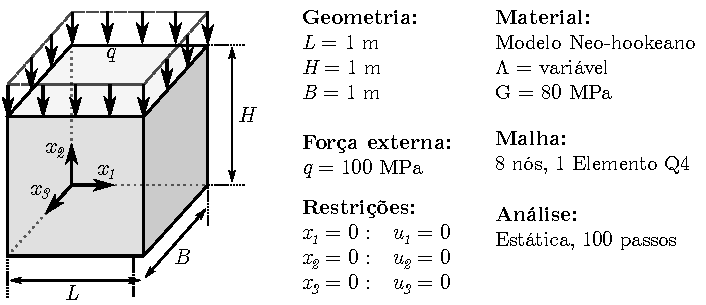
\includegraphics[scale=1.0]{Figuras/SimpleAxialCube3D/SimpleAxialCube3D.pdf}
					\end{center}\par}
				\vspace{-0.2cm}
			}
		}
	}	
	%\caption*{\textbf{Fonte:} Elaborado pelo autor}
\end{figure}

Na \autoref{fig:SimpleAxialCube3D-config} são mostradas as configurações deformadas finais para alguns casos analisados, possibilitando uma identificação visual da diferença entre os modelos, especialmente em relação ao volume obtido. 

\begin{figure}[!h]
	\centering
	\caption{Configurações deformadas finais para os casos com (a) $\Lambda = 10^0$ MPa, (b) $\Lambda = 10^2$ MPa e (c) modelo incompressível}
	\label{fig:SimpleAxialCube3D-config}
	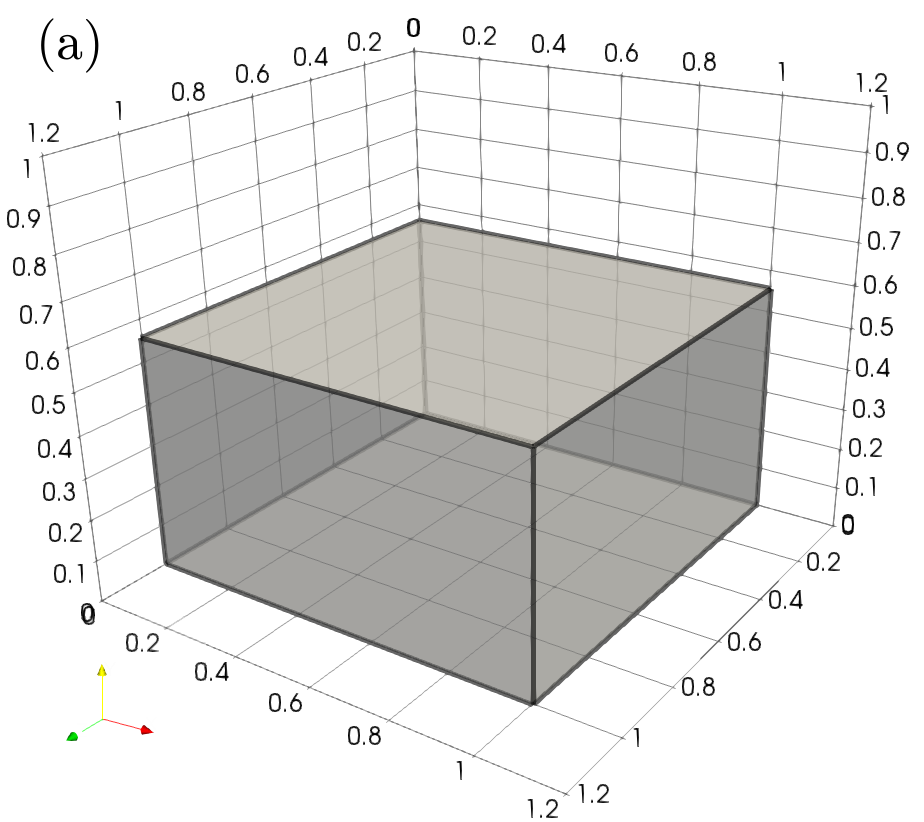
\includegraphics[scale=0.16]{Figuras/SimpleAxialCube3D/SimpleAxialCube3D-e0.png}\;\;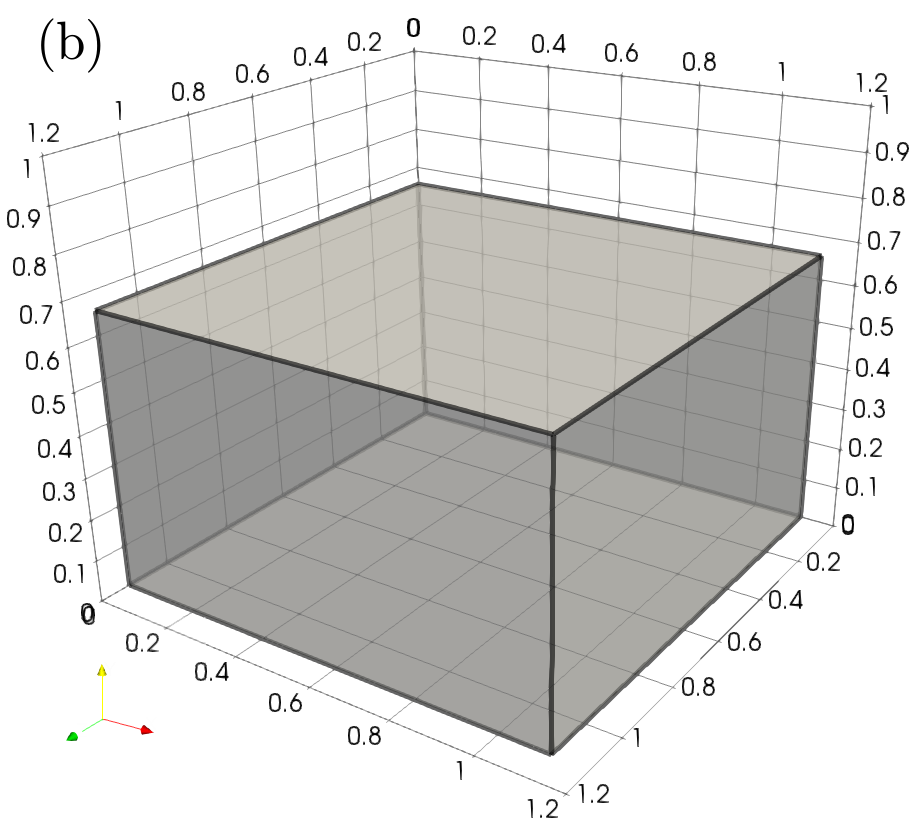
\includegraphics[scale=0.16]{Figuras/SimpleAxialCube3D/SimpleAxialCube3D-e2.png}\;\;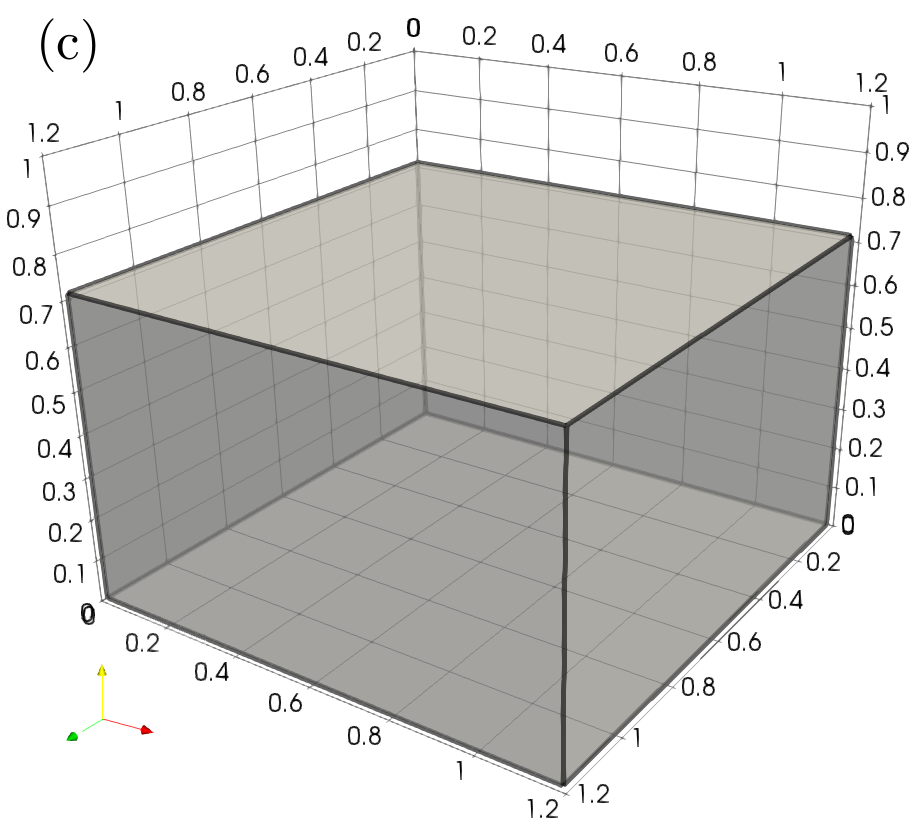
\includegraphics[scale=0.16]{Figuras/SimpleAxialCube3D/SimpleAxialCube3D-Incompressivel.png}
	%\caption*{\textbf{Fonte:} Elaborado pelo autor}
\end{figure}

Na \autoref{fig:SimpleAxialCube3D-Disp} são mostrados o gráficos de deslocamento horizontal e vertical por força aplicada, na \autoref{fig:SimpleAxialCube3D-Stress}(a) são mostrados os gráficos de tensão de Cauchy uniaxial, e na \autoref{fig:SimpleAxialCube3D-Stress}(b) são mostrados o gráficos de pressão por força aplicada. Para o modelo compressível, considera-se como pressão a parcela volumétrica da tensão, isto é, $\p = \lame\ln(\J)$. 

É possível observar nesses gráficos que o modelo compressível apresenta uma tendência ao modelo incompressível à medida que o valor de $\lame$ aumenta, conforme comentado no início deste capítulo. Particularmente para o presente problema, verifica-se que o modelo compressível com $\lame=10^4$ MPa já se mostra suficiente para simular o caso incompressível com um certo grau de precisão.

\begin{figure}[!h]
	\centering
	\caption{Gráficos de (a) deslocamento vertical por força aplicada e (b) deslocamento horizontal/vertical por força aplicada}
	\label{fig:SimpleAxialCube3D-Disp}
	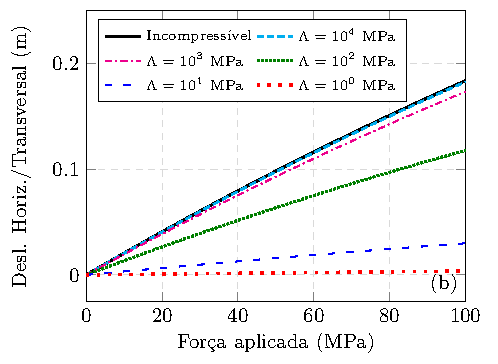
\includegraphics[scale=0.95]{Figuras/SimpleAxialCube3D/SimpleAxialCube3D-HorizontalDisp.pdf}\;\;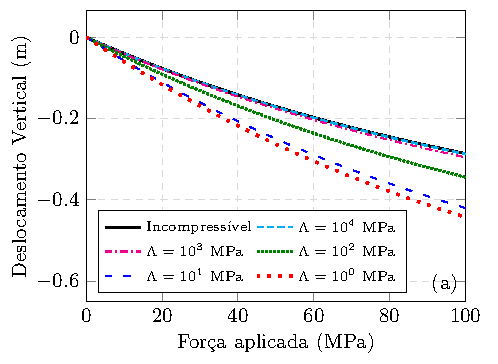
\includegraphics[scale=0.95]{Figuras/SimpleAxialCube3D/SimpleAxialCube3D-VerticalDisp.pdf}
	%\caption*{\textbf{Fonte:} Elaborado pelo autor}
\end{figure}

\begin{figure}[!h]
	\centering
	\caption{Gráficos de (a) tensão de Cauchy uniaxial por força aplicada e (b) pressão por força aplicada}
	\label{fig:SimpleAxialCube3D-Stress}
	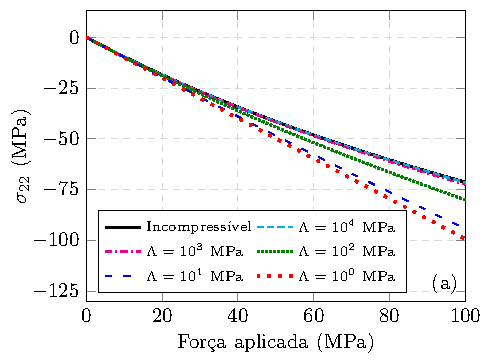
\includegraphics[scale=0.95]{Figuras/SimpleAxialCube3D/SimpleAxialCube3D-CauchyStress.pdf}\;\;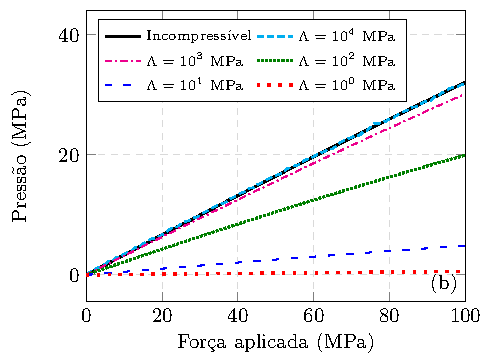
\includegraphics[scale=0.95]{Figuras/SimpleAxialCube3D/SimpleAxialCube3D-Pressure.pdf}
	%\caption*{\textbf{Fonte:} Elaborado pelo autor}
\end{figure}

Na \autoref{fig:SimpleAxialCube3D-Jacobian} é feita uma análise do Jacobiano para todos os casos analisados. A partir da \autoref{fig:SimpleAxialCube3D-Jacobian}(a) pode-se observar, como esperado, que o modelo incompressível resulta em Jacobiano unitário, e modelos compressíveis se distanciam mais desse valor à medida que $\lame$ diminui. Na \autoref{fig:SimpleAxialCube3D-Jacobian}(b) é apresentado um gráfico de convergência para o Jacobiano dos modelos compressíveis, considerando sua diferença com relação ao caso incompressível.

\begin{figure}[!h]
	\centering
	\caption{Gráficos de (a) Jacobiano por força aplicada e (b) $|J-1|$ por $\Lambda$ para os modelos compressíveis}
	\label{fig:SimpleAxialCube3D-Jacobian}
	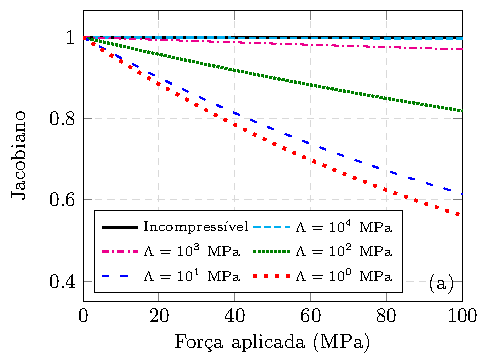
\includegraphics[scale=0.95]{Figuras/SimpleAxialCube3D/SimpleAxialCube3D-Jacobian.pdf}\;\;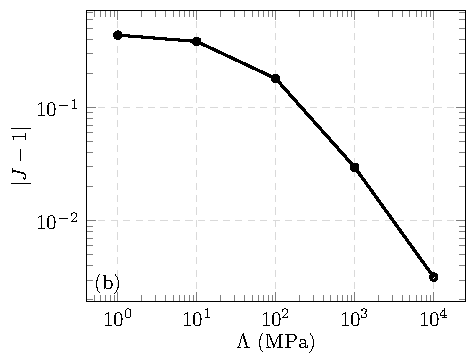
\includegraphics[scale=0.95]{Figuras/SimpleAxialCube3D/SimpleAxialCube3D-JacobianDifference.pdf}
	%\caption*{\textbf{Fonte:} Elaborado pelo autor}
\end{figure}

\section{Fluidos Newtonianos incompressíveis}\label{sec:incompressivelFluido}

Ao contrário de sólidos, fluidos não apresentam resistência a cisalhamento e podem deformar-se indefinidamente, facilmente levando a grandes mudanças topológicas, incluindo, por exemplo, separação e junção de subdomínios. Por esse motivo, formulações Lagrangianas como a apresentada neste capítulo podem não ser capazes de simular determinados problemas, sendo limitadas a certos casos onde não hajam mudanças topológicas excessivas.

Neste trabalho, aplica-se o modelo de fluido Newtoniano. Comumente utilizado no contexto Euleriano, o modelo original relaciona tensões de Cauchy com as taxas de deformação linear, sendo necessárias determinadas manipulações algébricas para escreve-lo em termos de grandezas Lagrangianas. A princípio, parte-se da relação
\begin{equation}\label{eq:newtonianFluid0}
\cauchyiso = 2\viscfluid\D,
\end{equation}
onde $\viscfluid$ é o parâmetro de viscosidade do fluido, $\cauchyiso$ é a parcela isocórica da tensão de Cauchy, e $\D$ é a taxa de deformação linear, também representada por $\dotDefLinear$.

Levando em conta a relação entre taxa de deformação linear e taxa de deformação de Green-Lagrange apresentada na \cref{eq:taxa-green-2}, e também a relação entre a tensão de Cauchy e a tensão de Piola-Kirchhoff de segunda espécie apresentada na \cref{eq:cauchy}, podemos representar a \cref{eq:newtonianFluid0} na forma
\begin{equation}\label{eq:newtonianFluid1}
\dfrac{1}{J}\F\Siso\F^T = 2\viscfluid\left(\F^{-T}\dotE\F^{-1}\right) \quad\Rightarrow\quad \Siso = 2\viscfluid\J\C^{-1}\dotE\C^{-1},
\end{equation}
isto é,
\begin{equation}\label{eq:newtonianFluid}
\Siso = \viscOperator:\dotE,
\end{equation}
onde $\viscOperator$, denominado operador de viscosidade, é um tensor de quarta ordem definido em forma indicial como
\begin{equation}
\viscOperator_{ijkl} = 2\viscfluid\J\left(\Cind^{-1}_{ik}\Cind^{-1}_{jl}\right).
\end{equation}

A taxa da deformação de Green-Lagrange pode ser calculada pela \cref{eq:dotE}, onde, no contexto do Método dos Elementos Finitos, calcula-se a taxa do gradiente da função mudança de configuração pela \cref{eq:dotF-FEM}.

Uma vez que este modelo constitutivo não é escrito apenas em termos da deformação de Green-Lagrange, mas também de sua taxa, algumas considerações adicionais devem ser feitas na formulação previamente apresentada. Em particular, a linearização das forças internas para solução do sistema não-linear pelo MEF, apresentada originalmente na \cref{eq:fint-lin}, deve ser reescrita como
\begin{equation}\label{eq:fint-lin2}
\dfrac{\partial \fint\nodeind}{\partial \y\nodeindDois_{\;\;\;}} = \int_{\domVoli}\left(\S:\dfrac{\partial^2\E_{\;}}{\partial\y\nodeind\otimes\y\nodeindDois} + \CC:\dfrac{\partial\E_{\;}}{\partial\y\nodeindDois}:\dfrac{\partial\E_{\;}}{\partial\y\nodeind} + \viscOperator:\dfrac{\partial\dotE_{\;}}{\partial\y\nodeindDois}:\dfrac{\partial\E_{\;}}{\partial\y\nodeind}\right)\,d\voli,
\end{equation}
onde o operador tangente consistente, $\CC$, é dado neste contexto por
\begin{equation}
\CC = \dfrac{\partial\S}{\partial\E} = 2\dfrac{\partial \viscOperator}{\partial\C}:\dotE
\text{\qquad ou \qquad} 
\CC_{ijkl} = \dfrac{\partial\Sind_{ij}}{\partial\Eind_{kl}} = 2\dfrac{\partial \viscOperator_{ijmn}}{\partial\Cind_{kl}}\dotEind_{mn},
\end{equation}
e a derivada da taxa da deformação de Green-Lagrange com relação às posições nodais pode ser calculada, a partir da \cref{eq:dotE-FEM}, como
\begin{equation}
\begin{aligned}
\dfrac{\partial\dotE_{\;}}{\partial\y\nodeindDois} &= \text{sim}\left(\Fini^{-T}\dfrac{\partial\dotFfin^{T}}{\partial\y\nodeindDois}\Ffin\Fini^{-1} + \Fini^{-T}\dotFfin^T\dfrac{\partial\Ffin}{\partial\y\nodeindDois}\Fini^{-1}\right) \\
&= \text{sim}\left(\Fini^{-T}\dfrac{\partial\dotFfin^{T}}{\partial\doty\nodeindDois}\Ffin\Fini^{-1}\right)\dfrac{\partial\doty\nodeindDois}{\partial\y\nodeindDois} + \text{sim}\left(\Fini^{-T}\dotFfin^T\dfrac{\partial\Ffin}{\partial\y\nodeindDois}\Fini^{-1}\right)\\
&=\dfrac{\partial\E}{\partial\y\nodeindDois}\dfrac{\partial\doty\nodeindDois}{\partial\y\nodeindDois} + \text{sim}\left(\Fini^{-T}\dotFfin^T\dfrac{\partial\Ffin}{\partial\y\nodeindDois}\Fini^{-1}\right),
\end{aligned}
\end{equation}
onde as derivadas ${\partial\E}/{\partial\y\nodeindDois}$ e ${\partial\Ffin}/{\partial\y\nodeindDois}$ são dadas nas \cref{eq:dE-dy,eq:dF1-dy}, respectivamente, e a derivada ${\partial\doty\nodeindDois}/{\partial\y\nodeindDois}$ depende do integrador temporal utilizado. Para o integrador Newmark-$\beta$, utilizado neste trabalho, calcula-se a partir da \cref{eq:vel}:
\begin{equation}
\dfrac{\partial\doty\nodeindDois}{\partial\y\nodeindDois} = \dfrac{\gammanewmark}{\betanewmark\Delta t}.
\end{equation}

\subsection{Tensão superficial}

A tensão superficial é um fenômeno físico que ocorre na interface entre um fluido (particularmente um líquido) e o meio externo. Esse fenômeno ocorre pois as moléculas da superfície não estão rodeadas por outras moléculas em todas as direções, como ocorre no interior do líquido. Consequentemente, elas são atraídas mais fortemente pelas moléculas adjacentes na interface e pelas moléculas internas. Essa atração desigual cria uma ``película'' na superfície do líquido, fazendo com que ele se comporte como se estivesse coberto por uma fina membrana elástica. A tensão superficial é responsável por diversos efeitos observáveis, como a formação de gotas esféricas, a capilaridade e a capacidade de alguns insetos caminharem sobre a água. 

Nesta seção, será utilizada como base a formulação descrita em \citeonline{saksono2002finite} e \citeonline{SaksonoPeric2006}. Como ilustrado na \cref{fig:SurfaceTension}, a tensão superficial atua como uma tensão de tração nas direções tangenciais à superfície do fluido. Embora parte dessa tensão se auto-equilibre, a presença de curvatura gera componentes que agem na direção normal à superfície, conforme representado na \cref{fig:SurfaceTension}(b) para o caso bidimensional. Assumindo uma tensão superficial $\surfaceTension$, é possível demonstrar que a componente normal da tensão atuante possui magnitude $2\surfaceTension\curvature$, onde $\curvature$ é a curvatura média da superfície, definida por:
\begin{equation}
\curvature = -\dfrac{1}{2}\gradientes\cdot\normalun = -\dfrac{1}{2}\left(\dfrac{\partial\normalunind_i}{\partial\yind_i} - \normalunind_i\normalunind_j\dfrac{\partial\normalunind_i}{\partial\yind_j} \right),
\end{equation}
sendo $\normalun$ o vetor normal unitário, definido conforme a \cref{sec:disc-contato}, e $\gradientes = (\I - \normalun\otimes\normalun)\gradiente$ o gradiente superficial ao longo da interface.

\begin{figure}[!htb]
	\centering
	\caption{Representação visual do fenômeno da tensão superficial}
	\label{fig:SurfaceTension}
	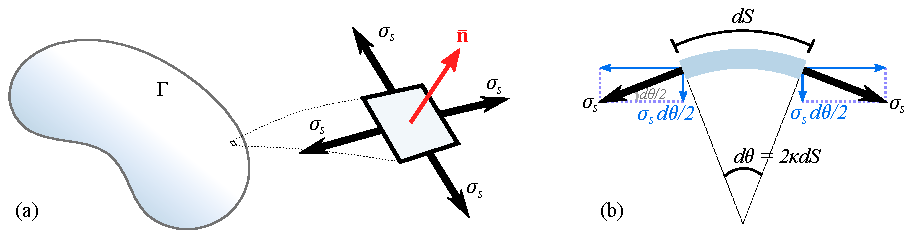
\includegraphics[scale=1]{Figuras/SurfaceTension.pdf}
	%\caption*{\textbf{Fonte:} Elaborado pelo autor}
\end{figure}

Utilizando a abordagem energética descrita na \cref{sec:equilibrio}, podemos incorporar essa tensão normal no problema mecânico como uma componente da energia potencial das forças externas. Sua variação pode ser expressa como
\begin{equation}\label{eq:surfacetension}
\delta\energiaextSurfaceTension = \int_{\domCon}2\surfaceTension\curvature\normal \cdot \delta\y\,d\con.
\end{equation}
Ao contrário das forças externas definidas na \cref{subsec:externas}, essa é não-conservativa, pois sua intensidade e direção variam ao longo do processo, de acordo com a geometria do domínio. Portanto, a \cref{eq:surfacetension} é integrada sobre o contorno deformado ($\domCon$) do fluido.

A \cref{eq:surfacetension} pode ser transformada utilizando o teorema da divergência, conforme detalhado em \citeonline{SaksonoPeric2006}. Isso resulta em
\begin{equation}\label{eq:surfacetension2}
\delta\energiaextSurfaceTension = -\int_{\domCon}\surfaceTension\gradientes\cdot \delta\y\,d\con + \int_{\domConn}\surfaceTension\binormal \cdot \delta\y\,d\conn,
\end{equation}
onde $\domConn$ representa o contorno de $\domCon$, e $\binormal$ denota o vetor binormal de $\domConn$, definido como o vetor tangente a $\domCon$ e ortogonal a $\domConn$. Para problemas tridimensionais, $\domCon$ é uma superfície bidimensional, enquanto $\domConn$ é uma curva. Já para problemas bidimensionais, $\domCon$ é uma curva, enquanto $\domConn$ é representada por pontos.

A forma apresentada na \cref{eq:surfacetension2} é vantajosa para aplicação no Método dos Elementos Finitos em comparação com a \cref{eq:surfacetension}, pois elimina a necessidade de calcular a curvatura. Isso viabiliza a utilização de elementos finitos lineares, nos quais a curvatura é localmente nula. Neste caso, o efeito da tensão superficial surge exclusivamente pela diferença de inclinação entre os elementos, que gera uma curvatura artificial e discreta ao longo do contorno.

Aplicando o MEF em conjunto com o método de Galerkin, a \cref{eq:surfacetension2} resulta em forças nodais, introduzidas no sistema como forças externas. Para cada nó $\node$ do contorno, essa força resultante é dada por
\begin{equation}\label{eq:surfacetensionforce}
(\fexts)\nodeind = -\int_{\domCon}\surfaceTension\gradientes\,\fforma\nodeind\,d\con + \int_{\domConn}\surfaceTension\binormal \fforma\nodeind\,d\conn,
\end{equation}
ou, em notação indicial,
\begin{equation}\label{eq:surfacetensionforce2}
(\fextsind)\nodeind_i = -\int_{\domCon}\surfaceTension\left(\dfrac{\partial\fforma\nodeind}{\partial\yind_i} - \normalunind_i\normalunind_j\dfrac{\partial\fforma\nodeind}{\partial\yind_j} \right)\,d\con + \int_{\domConn}\surfaceTension\binormalind_i \fforma\nodeind\,d\conn.
\end{equation}
As derivadas das funções de forma com relação às posições podem ser calculadas utilizando a regra da cadeia, isto é:
\begin{equation}
\dfrac{\partial\fforma\nodeind}{\partial\y} = \dfrac{\partial\fforma\nodeind}{\partial\coords} \cdot \dfrac{\partial\coords}{\partial\y},
\end{equation}
onde ${\partial\coords}/{\partial\y}$ é dado pela inversa de $\Ffin = {\partial\y}/{\partial\coords}$. Para esse cálculo, uma particularidade deve ser levada em conta: dado que $\domCon$ é uma superfície bidimensional imersa em um espaço tridimensional (no caso 3D), ou uma curva unidimensional imersa em um espaço bidimensional (no caso 2D), $\Ffin$ não é uma matriz quadrada, mas sim uma matriz com dimensões $3\times 2$ ou $2\times 1$. Assim, o conceito convencional de matriz inversa é substituído pela pseudoinversa de Moore-Penrose, e ${\partial\coords}/{\partial\y}$ é calculado como:
\begin{equation}\label{eq:dksi_dy}
\dfrac{\partial\coords}{\partial\y} = (\Ffin^T\Ffin)^{-1}\Ffin^T.
\end{equation}
No caso 2D, onde a coordenada adimensional é um escalar, e $\Ffin$ possui dimensões $2\times 1$, a \cref{eq:dksi_dy} pode ser simplificada para
\begin{equation}\label{eq:dksi_dy2D}
\dfrac{\partial\coordsind}{\partial\y} = \dfrac{\partial\y}{\partial\coordsind}\left\Vert\dfrac{\partial\y}{\partial\coordsind}\right\Vert^{-\frac{1}{2}}.
\end{equation}

\subsubsection{Forças resultantes em elementos isolados e análise de pontos de integração}\label{subsec:forcas-tensao-residual}

As integrais apresentadas nas \cref{eq:surfacetensionforce,eq:surfacetensionforce2} são calculadas numericamente utilizando quadraturas adequadas ao tipo de elemento finito empregado. Devido à alta não-linearidade das expressões integradas, especialmente em elementos de alta ordem, sabe-se que esse processo produz resultados aproximados, sendo mais precisos quanto maior o número de pontos de integração. No entanto, o aumento desse número também resulta em um maior tempo de processamento. Para garantir uma relação ótima entre precisão e custo computacional, é realizada nesta seção uma análise para definir o número ideal de pontos de integração em cada tipo de elemento utilizado.

Para problemas bidimensionais, onde $\domCon$ é unidimensional, consideram-se elementos de curva (ou de linha) com $2$, $3$ e $4$ nós, denotados por L2, L3, e L4, respectivamente. Esses elementos possuem aproximações linear, quadrática, e cúbica, nessa ordem, sendo utilizada a quadratura de Gauss para integrar ao longo de seus domínios.

A quantidade necessária de pontos de integração é dependente da disposição geométrica do elemento, incluindo fatores como curvatura e variação do vetor normal. Uma vez que esses fatores são variáveis ao longo do problema, considera-se nesta análise um caso extremo onde o elemento forma um quadrante de circunferência. Entretanto, na prática, recomenda-se discretizar o problema suficientemente para que a disposição geométrica individual de cada elemento finito não ultrapasse esse caso extremo. Naturalmente, esse quadrante será aproximado por polinômios, com fidelidade geométrica limitada pela ordem do elemento finito. 

Tomando-se um elemento com tensão superficial unitária, calcula-se, para cada um de seus nós, a força resultante através da primeira integral da \cref{eq:surfacetensionforce}. A segunda integral é desprezada neste contexto pois assume-se que o elemento não intersecta o contorno de $\domCon$. As coordenadas dos nós e as forças nodais resultantes, utilizando $20$ pontos de integração, são apresentadas na \cref{tab:SurfaceTensionTest-nodes-1} para cada tipo de elemento de curva considerado, sendo representadas visualmente na \cref{fig:SurfaceTensionTest-Paraview-curve}.

\begin{table}[!htb]
	\centering
	\caption{Coordenadas e forças resultantes em nós de elementos de curva sujeitos a tensão superficial, utilizando $20$ pontos de integração da quadratura de Gauss}
	\scriptsize
	\label{tab:SurfaceTensionTest-nodes-1}
	{\def\arraystretch{2}
		\begin{tabular}{ll}
			\multicolumn{2}{c}{(a) L2} \\ \hline
			Coords. & Força nodal result. \\ \hline
			$\left( 0; 1 \right)$ & $\left( 0.707107; -0.707107 \right)$ \\
			$\left( 1; 0 \right)$ & $\left( -0.707107; 0.707107 \right)$ \\ \hline
			& \\
			& \\
			& \\[0.25cm]
		\end{tabular}\;
		\begin{tabular}{ll}
			\multicolumn{2}{c}{(b) L3} \\ \hline
			Coords. & Força nodal result. \\ \hline
			$\Big( 0; 1 \Big)$ & $\left( 0.974986; -0.313389 \right)$ \\
			$\Big( \frac{\sqrt{2}}{2}; \frac{\sqrt{2}}{2} \Big)$ & $\left( -0.66160; -0.66160 \right)$ \\
			$\Big( 1; 0 \Big)$ & $\left( -0.313389; 0.974986 \right)$ \\ \hline
			& \\
			& \\[0.17cm]
		\end{tabular}\;
		\begin{tabular}{ll}
			\multicolumn{2}{c}{(c) L4} \\ \hline
			Coords. & Força nodal result. \\ \hline
			$\Big( 0; 1 \Big)$ & $\left( 0.9621; -0.179398 \right)$ \\
			$\Big( \frac{1}{2}; \frac{\sqrt{3}}{2} \Big)$ & $\left( -0.19446; -0.58824 \right)$ \\
			$\Big( \frac{\sqrt{3}}{2}; \frac{1}{2} \Big)$ & $\left( -0.58824; -0.19446 \right)$ \\
			$\Big( 1; 0 \Big)$ & $\left( -0.179398; 0.9621 \right)$ \\ \hline
			& \\[0.15cm]
		\end{tabular}
	}
	%\caption*{\textbf{Fonte:} Elaborado pelo autor}
\end{table}

\begin{figure}[!htb]
	\centering
	\caption{Representação visual de elementos de curva utilizados em análise de pontos de integração para tensão superficial}
	\label{fig:SurfaceTensionTest-Paraview-curve}
	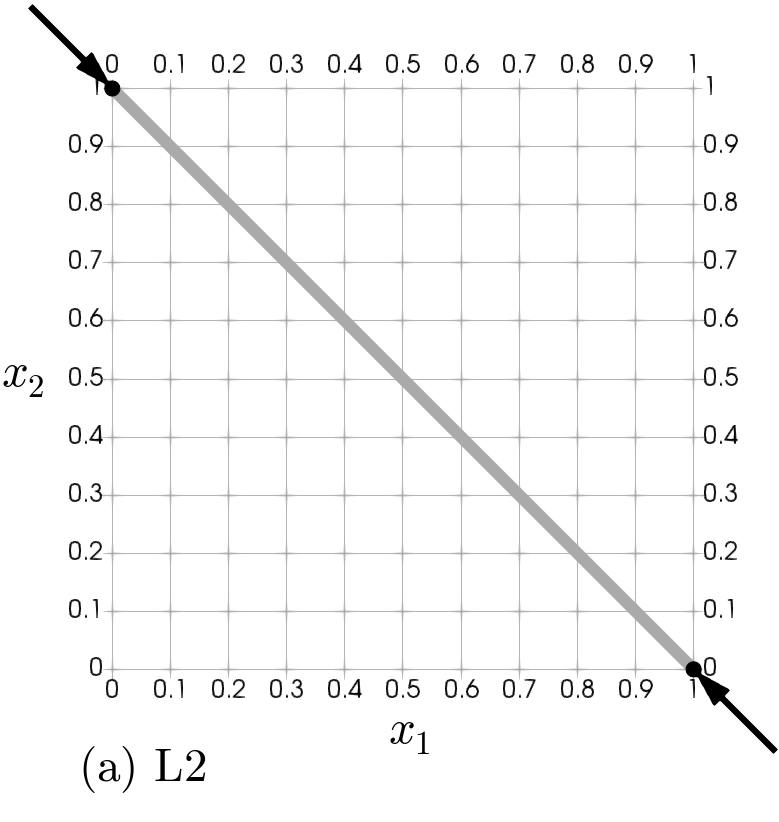
\includegraphics[scale=0.25]{Figuras/SurfaceTensionTest/Paraview/L2.png}\quad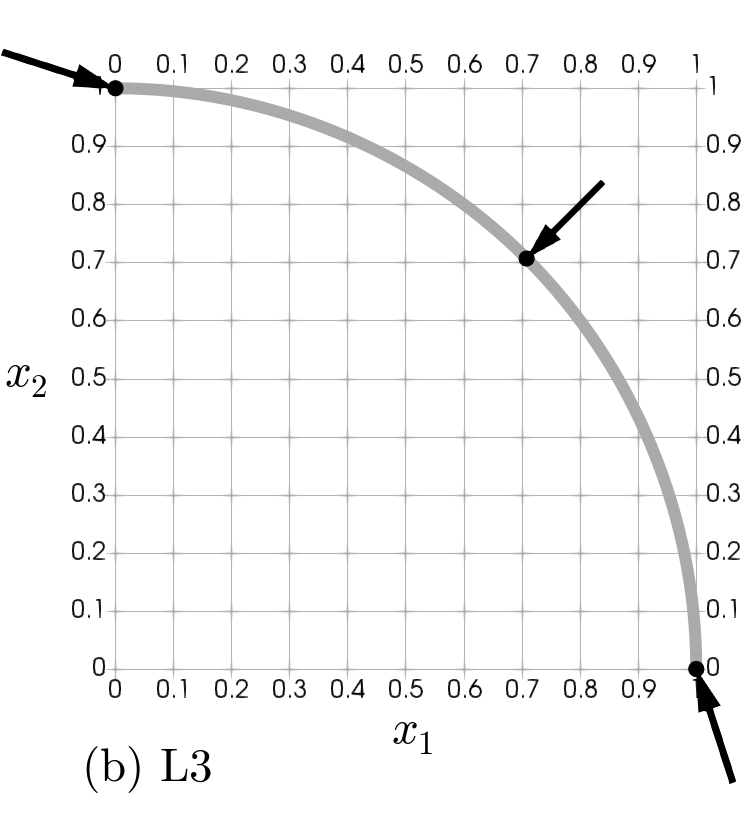
\includegraphics[scale=0.25]{Figuras/SurfaceTensionTest/Paraview/L3.png}\quad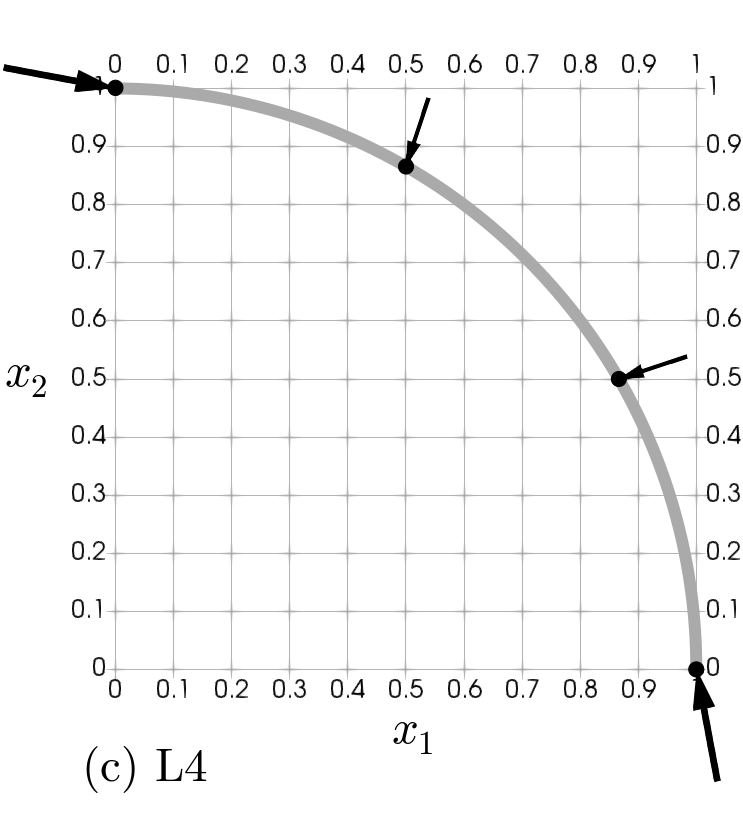
\includegraphics[scale=0.25]{Figuras/SurfaceTensionTest/Paraview/L4.png}
	%\caption*{\textbf{Fonte:} Elaborado pelo autor}
\end{figure}

Para problemas tridimensionais, onde $\domCon$ é bidimensional, consideram-se os elementos triangulares T3, T6 e T10, com aproximações linear, quadrática, e cúbica, respectivamente. A integração numérica neste caso é feita utilizando a quadratura de \citeonline{dun85}, que possui um número máximo de $79$ pontos de integração.

Neste caso, assumem-se elementos que simulam a disposição geométrica de um octante de uma esfera. As coordenadas dos nós e as forças resultantes, utilizando $79$ pontos de integração, são dispostas na \cref{tab:SurfaceTensionTest-nodes-2}, com representação visual de cada caso apresentada na \cref{fig:SurfaceTensionTest-Paraview}.

\begin{table}[!htb]
	\centering
	\caption{Coordenadas e forças resultantes em nós de elementos triangulares sujeitos a tensão superficial, utilizando $79$ pontos de integração da quadratura de Dunavant}
	\scriptsize
	\label{tab:SurfaceTensionTest-nodes-2}
	{\def\arraystretch{2}
		\begin{tabular}{ll}
			\multicolumn{2}{c}{(a) T3} \\ \hline
			Coordenadas & Força nodal resultante \\ \hline
			$\left(0; 0; 1\right)$  & $\left(0.288675; 0.288675; -0.57735\right)$  \\
			$\left(0; 1; 0\right)$ & $\left(0.288675; -0.57735; 0.288675\right)$ \\
			$\left(1; 0; 0\right)$ & $\left(-0.57735; 0.288675; 0.288675\right)$ \\ \hline
			& \\[-0.5cm]
			\multicolumn{2}{c}{(b) T6} \\ \hline
			Coordenadas & Força nodal resultante \\ \hline
			$\Big(0; 0; 1\Big)$ & $\left(0,299576; 0,299576; -0,169459\right)$ \\
			$\left(0; \frac{\sqrt{2}}{2}; \frac{\sqrt{2}}{2}\right)$ & $\left(0,687796; -0,558743; -0,558743\right)$ \\
			$\Big(0; 1; 0\Big)$ & $\left(0,299574; -0,169459; 0,299576\right)$ \\
			$\left(\frac{\sqrt{2}}{2}; 0; \frac{\sqrt{2}}{2}\right)$ & $\left(-0,558743; 0,687796; -0,558743\right)$ \\
			$\left(\frac{\sqrt{2}}{2}; \frac{\sqrt{2}}{2}; 0\right)$ & $\left(-0,558744; -0,558744; 0,687795\right)$ \\
			$\Big(1; 0; 0\Big)$ & $\left(-0,169459; 0,299574; 0,299576\right)$ \\ \hline
		\end{tabular}\qquad
		\begin{tabular}{ll}
			\multicolumn{2}{c}{(c) T10} \\ \hline
			Coordenadas & Força nodal resultante \\ \hline
			$\Big(0; 0; 1\Big)$  & $\left(0,175642; 0,175642; -0,0113901\right)$  \\
			$\left(0; \frac{1}{2}; \frac{\sqrt{3}}{2}\right)$ & $\left(0.589651; 0,00375044; -0,253053\right)$ \\
			$\left(0; \frac{\sqrt{3}}{2}; \frac{1}{2}\right)$ & $\left(0.572785; -0,299737; -0,0255342\right)$ \\
			$\Big(0; 1; 0\Big)$ & $\left(0,157543; -0,0733659; 0,153388\right)$ \\
			$\left(\frac{1}{2}; 0; \frac{\sqrt{3}}{2}\right)$ & $\left(0,00375044; 0.589651; -0,253053\right)$ \\
			$\left(\frac{1}{2}; \frac{1}{2}; \frac{\sqrt{2}}{2}\right)$ & $\left(-0,691797; -0,691797; -0,83786\right)$ \\
			$\left(\frac{1}{2}; \frac{\sqrt{3}}{2}; 0\right)$ & $\left(-0,0757699; -0,358703; 0.549825\right)$ \\
			$\left(\frac{\sqrt{3}}{2}; 0; \frac{1}{2}\right)$ & $\left(-0,299737; 0.572785; -0,0255342\right)$ \\
			$\left(\frac{\sqrt{3}}{2}; \frac{1}{2}; 0\right)$ & $\left(-0,358703; -0,0757699; 0.549825\right)$ \\
			$\Big(1; 0; 0\Big)$ & $\left(-0,0733659; 0,157543; 0,153388\right)$ \\ \hline
			& \\[0.15cm]
		\end{tabular}
	}
	%\caption*{\textbf{Fonte:} Elaborado pelo autor}
\end{table}

\begin{figure}[!htb]
	\centering
	\caption{Representação visual de elementos triangulares utilizados em análise de pontos de integração para tensão superficial}
	\label{fig:SurfaceTensionTest-Paraview}
	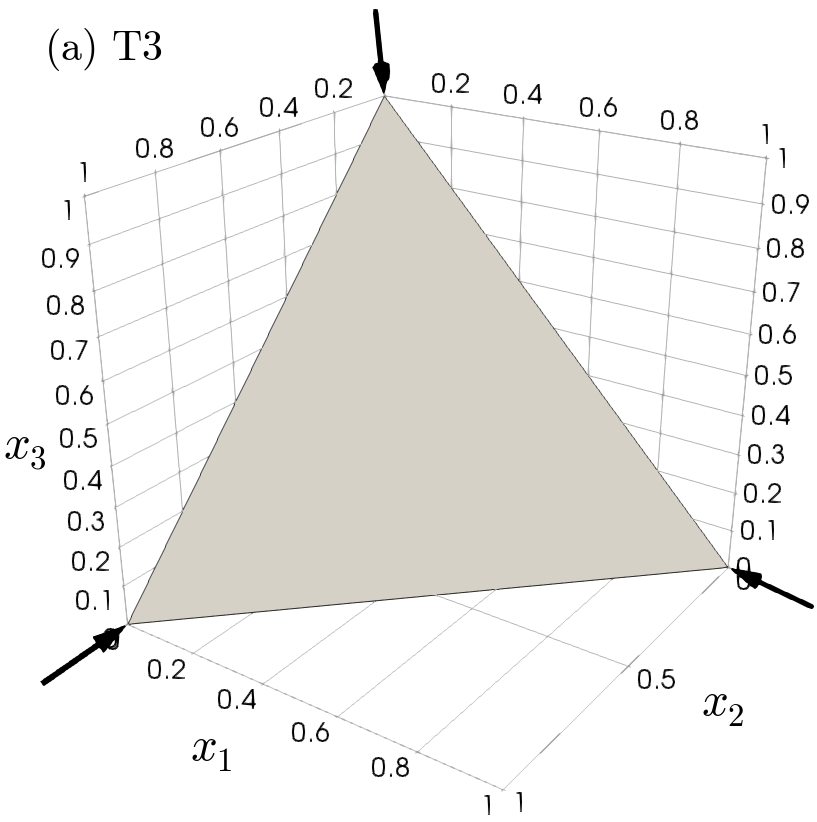
\includegraphics[scale=0.235]{Figuras/SurfaceTensionTest/Paraview/T3.png}\quad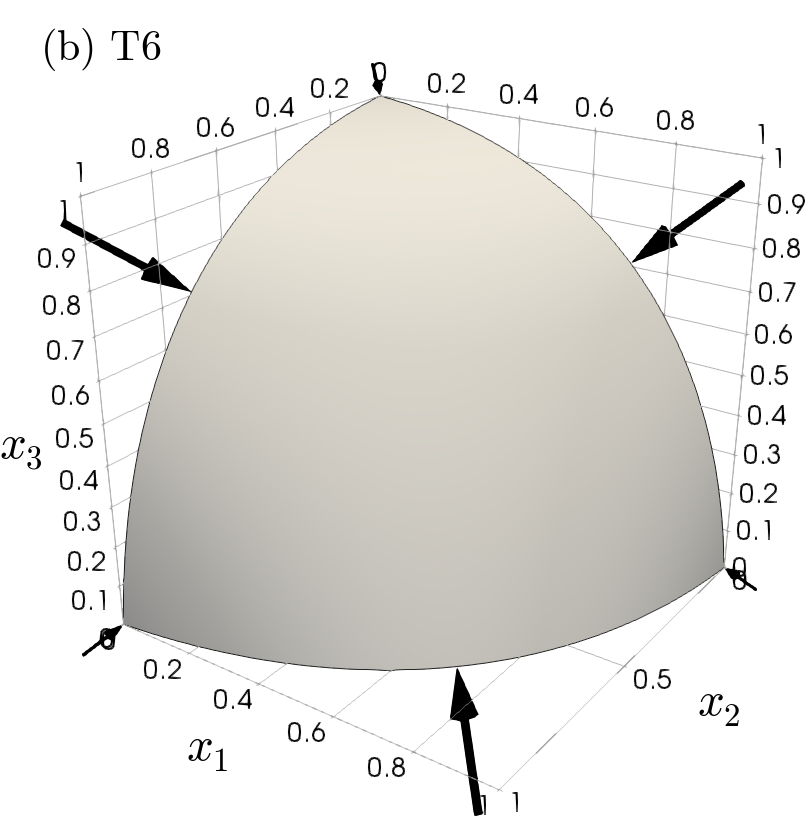
\includegraphics[scale=0.235]{Figuras/SurfaceTensionTest/Paraview/T6.png}\quad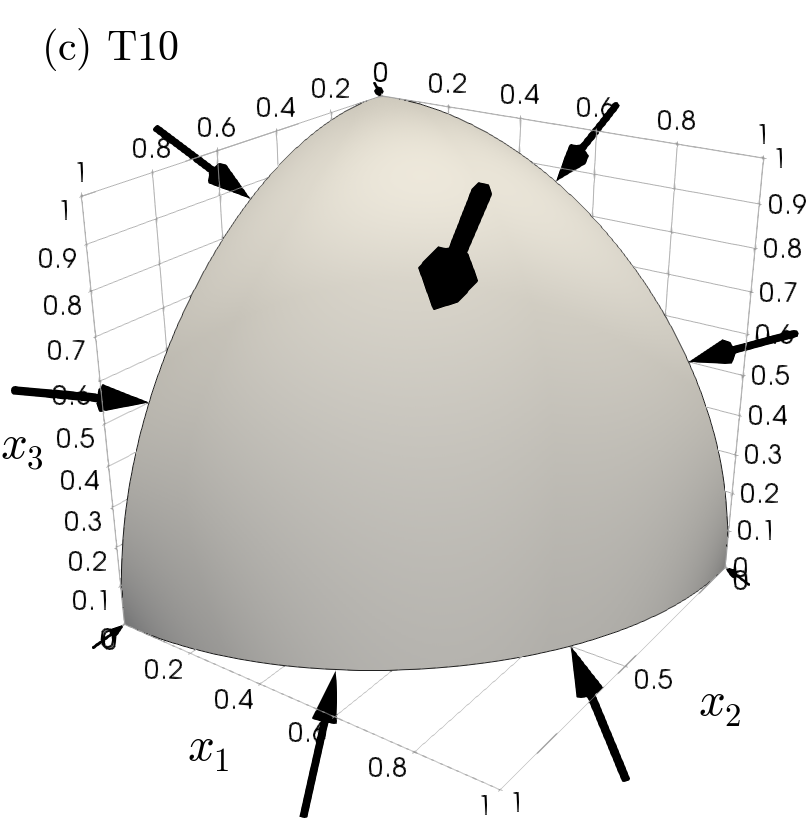
\includegraphics[scale=0.235]{Figuras/SurfaceTensionTest/Paraview/T10.png}
	%\caption*{\textbf{Fonte:} Elaborado pelo autor}
\end{figure}


Observa-se que os nós centrais dos elementos possuem forças resultantes mais próximas da direção normal, enquanto os nós de bordo exibem forças mais próximas da direção tangente. Entretanto, os nós de bordo recebem ainda contribuições similares de elementos vizinhos, fazendo com que a força resultante se alinhe com a bissetriz entre os elementos. Esse efeito permite que a diferença de inclinação entre elementos adjacentes seja tratada como uma curvatura artificial, apesar da falta de suavidade geométrica. Considere, por exemplo, um nó de canto que conecta elementos de linha retos e perpendiculares entre si, conforme ilustrado na \cref{fig:SurfaceTension2}. Nesse caso, a soma das forças resultantes no nó em cada elemento produzirá uma força inclinada a 45$^{\circ}$ (bissetriz).

\begin{figure}[!htb]
	\centering
	\caption{Representação de força resultante de tensão superficial em nó de canto}
	\label{fig:SurfaceTension2}
	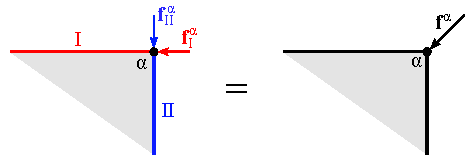
\includegraphics[scale=1.4]{Figuras/SurfaceTension2.pdf}
	%\caption*{\textbf{Fonte:} Elaborado pelo autor}
\end{figure}

Esse comportamento causa uma tendência a suavizar os cantos do domínio. Por esse motivo, líquidos que não estão sujeitos a outras forças além da tensão superficial tendem a assumir um formato esférico. Em geral, a tensão superficial atua de forma a minimizar a área da superfície para um determinado volume.

Seguindo para a análise de pontos de integração, calculamos as forças resultantes em cada um dos elementos finitos previamente apresentados, utilizando números menores de pontos de integração. Para os elementos de curva, empregamos de 1 a 19 pontos da quadratura de Gauss, comparando-os com a referência de 20 pontos (\cref{tab:SurfaceTensionTest-nodes-1}). Nos elementos triangulares, utilizamos de 1 a 73 pontos da quadratura de \citeonline{dun85}, comparando-os com a referência de 79 pontos (\cref{tab:SurfaceTensionTest-nodes-2}). 

O erro em cada nó $\alpha$ é calculado por $e^{\alpha} = \|\mathbf{f}^{\alpha} - \mathbf{f}^{\alpha}_\text{ref}\|/\|\mathbf{f}^{\alpha}_\text{ref}\|$, onde $\mathbf{f}^{\alpha}$ representa a força resultante calculada e $\mathbf{f}^{\alpha}_\text{ref}$ a força de referência. O erro total no elemento é determinado pela fórmula $e = \sqrt{\sum{\alpha} (e^{\alpha})^2}$. A \cref{fig:SurfaceTensionTest-Errors} mostra os gráficos dos erros em função do número de pontos de integração para cada tipo de elemento.

\begin{figure}[!htb]
	\centering
	\caption{Análise de convergência de pontos de integração para tensão superficial em (a) elementos de curva e (b) elementos triangulares}
	\label{fig:SurfaceTensionTest-Errors}
	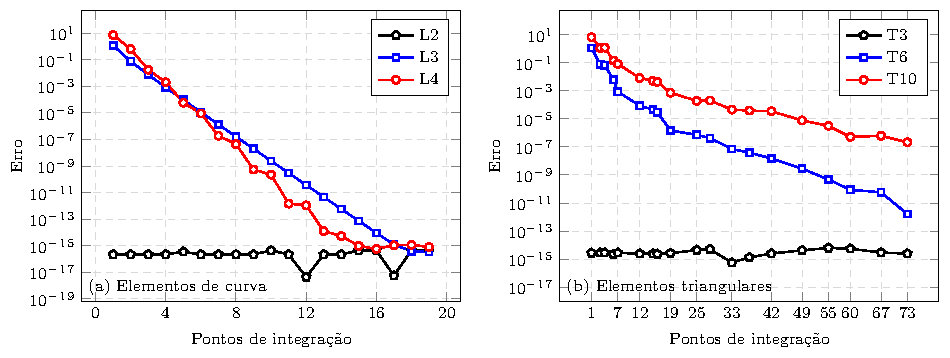
\includegraphics[scale=1.0]{Figuras/SurfaceTensionTest/SurfaceTensionTest-Errors.pdf}
	%\caption*{\textbf{Fonte:} Elaborado pelo autor}
\end{figure}

Destaca-se que os elementos de ordem linear, como o L2 e o T3, não são afetados pelo número de pontos de integração. Uma vez que o vetor normal e a inclinação são constantes ao longo desses elementos, a resposta numérica exata da \cref{eq:surfacetensionforce2} é obtida com apenas $1$ ponto de integração. Por esse motivo, os erros associados a esses elementos na \cref{fig:SurfaceTensionTest-Errors} são mínimos, equivalentes a resíduos computacionais. Por outro lado, os elementos de ordem quadrática e cúbica apresentam um comportamento convergente, com os erros diminuindo progressivamente à medida que o número de pontos de integração aumenta.

Utilizando os gráficos da \cref{fig:SurfaceTensionTest-Errors} como referência, pode-se estabelecer um critério de tolerância para o erro, de acordo com o nível de precisão almejado para as forças resultantes. Neste trabalho, utiliza-se o critério $e < 10^{-3}$, culminando nos pontos de integração dispostos na \cref{tab:SurfaceTensionTest-points}.

\begin{table}[!htb]
	\centering
	\caption{Pontos de integração selecionados para tensão superficial em diversos tipos de elementos, utilizando o critério $e < 10^{-3}$}
	\footnotesize
	\label{tab:SurfaceTensionTest-points}
	{\renewcommand{\arraystretch}{1.1}
		\begin{tabular}{C{1cm} C{1cm} C{1cm} C{1cm} C{1cm} C{1cm}}
			\hline
			\rowcolor{LightGray}
			\multicolumn{3}{c}{Elementos de curva} & \multicolumn{3}{c}{Elementos triangulares}\\
			\rowcolor{LightGray} L2 & L3 & L4 & T3 & T6 & T10  \\  \hline
			$1$ & $4$ & $5$ & $1$ & $7$ & $19$  \\ \hline
		\end{tabular}
	}
	%\caption*{\textbf{Fonte:} Elaborado pelo autor}
\end{table}

Vale ressaltar que esta análise considera elementos sujeitos a um alto grau de variação geométrica ao longo de seu domínio (\cref{fig:SurfaceTensionTest-Paraview-curve,fig:SurfaceTensionTest-Paraview}), o que não é comum em problemas com malhas suficientemente refinadas. Em situações usuais, os erros obtidos com os pontos de integração da \cref{tab:SurfaceTensionTest-points} podem ser muito inferiores ao critério de $10^{-3}$ estabelecido.

\subsection{Exemplos numéricos de fluidos}

A seguir, são apresentados exemplos numéricos com o objetivo de verificar o modelo implementado de fluido Newtoniano incompressível.

\subsubsection{\emph{Sloshing} de pequena amplitude}

Este exemplo consiste de um tanque de água cujas condições iniciais são representadas na \autoref{fig:FluidSlosh}, sendo adotada condição de deslizamento nas paredes. Duas malhas são consideradas: a primeira formada por elementos T3, e a segunda por elementos T10. Não foi necessário aplicar a estabilização neste caso.

\begin{figure}[!htb]
	\centering
	\caption{Geometria e dados do exemplo: \emph{Sloshing} de pequena amplitude}
	\label{fig:FluidSlosh}
	{\small
		\noindent\shadowbox{
			\parbox{15.3cm}{
				\setlength{\columnseprule}{1pt}
				\vspace{-0.2cm}
				{\centering\begin{center}
					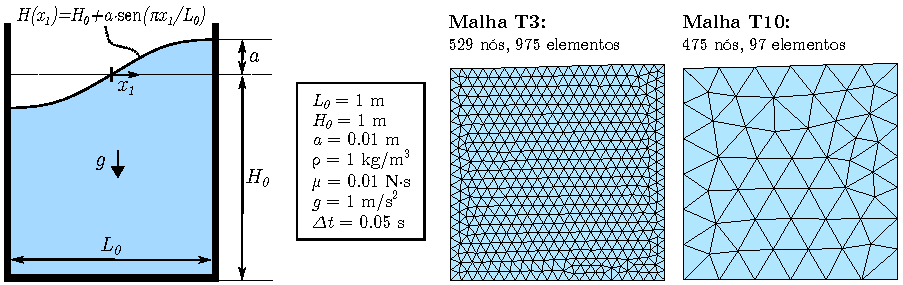
\includegraphics[scale=0.98]{Figuras/FluidSlosh/FluidSlosh.pdf}
					\end{center}\par}
				\vspace{-0.2cm}
			}
		}
	}	
	%\caption*{\textbf{Fonte:} Elaborado pelo autor}
\end{figure}

Por ser um exemplo com baixos níveis de deformação, sua simulação foi possível com a formulação apresentada do Método dos Elementos Finitos, mostrando resultados consistentes com a literatura. Na \autoref{fig:FluidSlosh-height} são apresentados os valores das alturas da superfície livre ao longo do tempo nas extremidades esquerda e direita do tanque, sendo observado um comportamento oscilatório. Esses resultados são similares para as duas malhas analisadas, mostrando ótima concordância com os de \citeonline{Avancini2020}.

\begin{figure}[!htb]
	\centering
	\caption{Altura da superfície livre nas extremidades esquerda e direita do recipiente com relação ao tempo}
	\label{fig:FluidSlosh-height}
	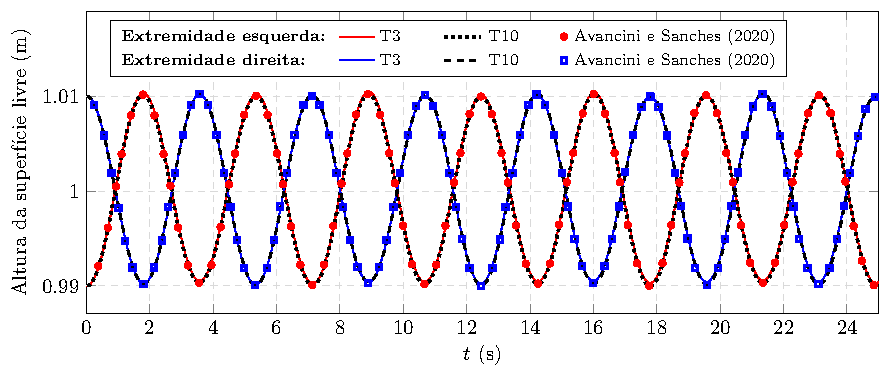
\includegraphics[scale=1.0]{Figuras/FluidSlosh/FluidSlosh-height.pdf}
	%\caption*{\textbf{Fonte:} Elaborado pelo autor}
\end{figure}

Nas \cref{fig:FluidSloshT3,fig:FluidSloshT10} são mostradas as configurações deformadas para ambas as malhas em determinados passos de tempo, onde é possível observar visualmente o comportamento oscilatório demonstrado na \autoref{fig:FluidSlosh-height}. Também são mostrados em mapas de cores os campos de pressão em cada caso. Por se tratar de um tanque com variações baixas na superfície livre, é possível observar que as pressões são aproximadamente constantes ao longo do seu comprimento, e variam de forma linear ao longo de sua altura, coincidindo com resultados clássicos da hidrodinâmica.

\begin{figure}[!htb]
	\centering
	\caption{Configurações deformadas para a malha T3, com pressão (Pa) em mapa de cores}
	\label{fig:FluidSloshT3}
	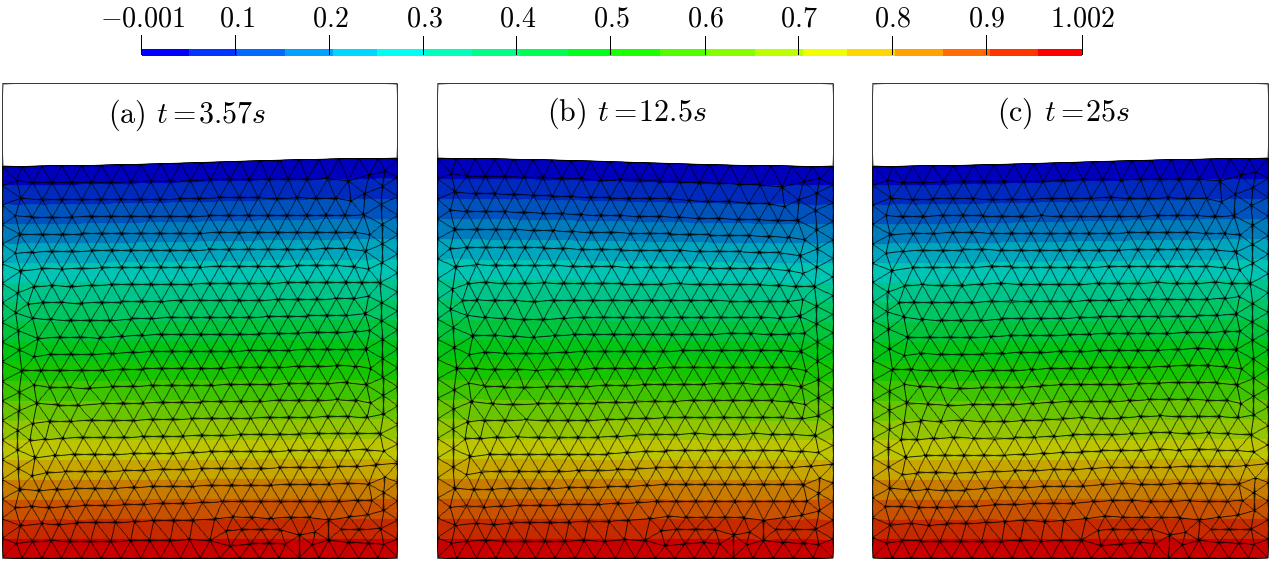
\includegraphics[scale=0.47]{Figuras/FluidSlosh/FluidSloshT3.png}
	%\caption*{\textbf{Fonte:} Elaborado pelo autor}
\end{figure}

\begin{figure}[!htb]
	\centering
	\caption{Configurações deformadas para a malha T10, com pressão (Pa) em mapa de cores}
	\label{fig:FluidSloshT10}
	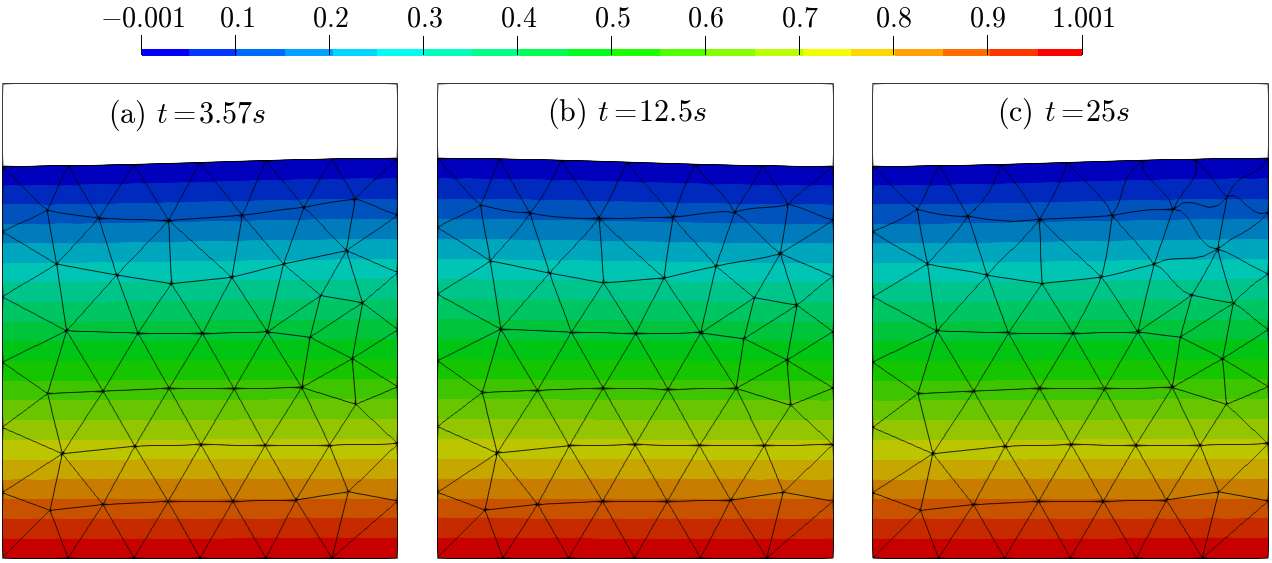
\includegraphics[scale=0.47]{Figuras/FluidSlosh/FluidSloshT10.png}
	%\caption*{\textbf{Fonte:} Elaborado pelo autor}
\end{figure}

\subsubsection{Colapso de barragem sob superfície lisa}\label{sec:barragem}

Neste exemplo, simula-se o colapso de uma coluna de água sob seu peso próprio, considerando os dados dispostos na \autoref{fig:FluidDam}. Novamente são consideradas malhas T3 e T10, e são adotadas condições de deslizamento na parede e no chão. Neste caso, foi necessária a estabilização PSPG para regularizar os campos de pressão encontrados, sendo o parâmetro $\multiplierpspg$ da \cref{eq:tpspg} tomado igual a $1$. Além disso, são adotados os parâmetros de \citeonline{Hu1997} para o integrador Newmark-$\beta$ a fim de dissipar as altas frequências obtidas: $\beta = 1$ e $\gamma = 1,5$.

\begin{figure}[!htb]
	\centering
	\caption{Geometria e dados do exemplo: colapso de barragem sob superfície lisa}
	\label{fig:FluidDam}
	{\small
		\noindent\shadowbox{
			\parbox{15.3cm}{
				\setlength{\columnseprule}{1pt}
				\vspace{-0.2cm}
				{\centering\begin{center}
					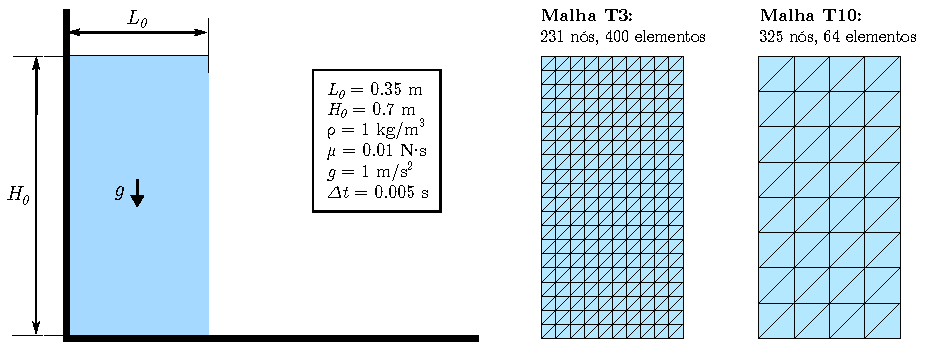
\includegraphics[scale=0.97]{Figuras/FluidDam/FluidDam.pdf}
					\end{center}\par}
				\vspace{-0.2cm}
			}
		}
	}	
	%\caption*{\textbf{Fonte:} Elaborado pelo autor}
\end{figure}

Apesar de ser um problema com grandes deformações, e que pode evoluir indefinidamente à medida que o tempo avança, é possível simula-lo de forma relativamente adequada com o Método dos Elementos Finitos, uma vez que não são identificadas mudanças excessivas na estrutura topológica da malha, como formação de vórtices e tentativas de separação de domínios. 

Nas \cref{fig:FluidDamT3,fig:FluidDamT10} são mostradas as configurações deformadas em determinados passos de tempo para ambas as malhas consideradas, sendo o tempo marcado em sua forma adimensional $t^* = t\sqrt{2g/L_0}$. Embora o comportamento geral do problema seja similar para ambos os casos, é possível observar que, nas presentes condições, o caso com elementos T10 apresentou resultados levemente mais regulares, sem oscilações geométricas da malha como as observadas na \autoref{fig:FluidDamT3}.

\begin{figure}[!htb]
	\centering
	\caption{Configurações deformadas para a malha T3, com pressão (Pa) em mapa de cores}
	\label{fig:FluidDamT3}
	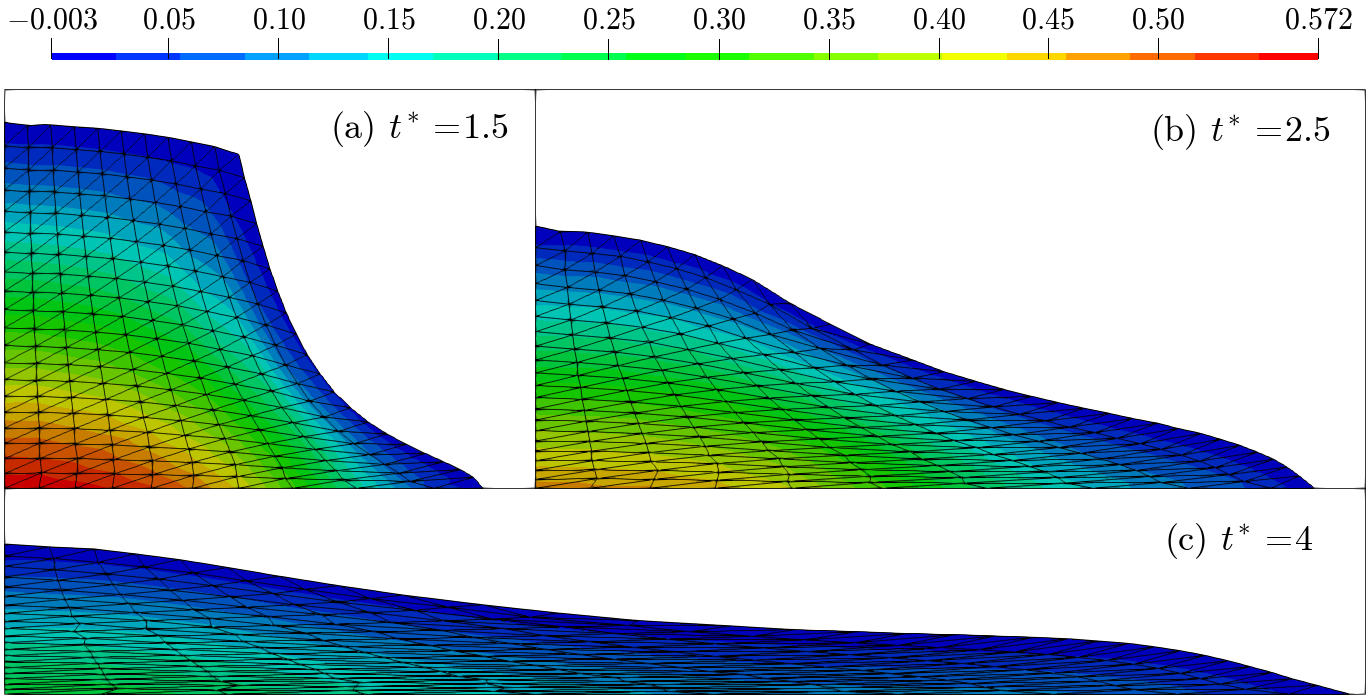
\includegraphics[scale=0.4]{Figuras/FluidDam/FluidDamT3.png}
	%\caption*{\textbf{Fonte:} Elaborado pelo autor}
\end{figure}

\begin{figure}[!htb]
	\centering
	\caption{Configurações deformadas para a malha T10, com pressão (Pa) em mapa de cores}
	\label{fig:FluidDamT10}
	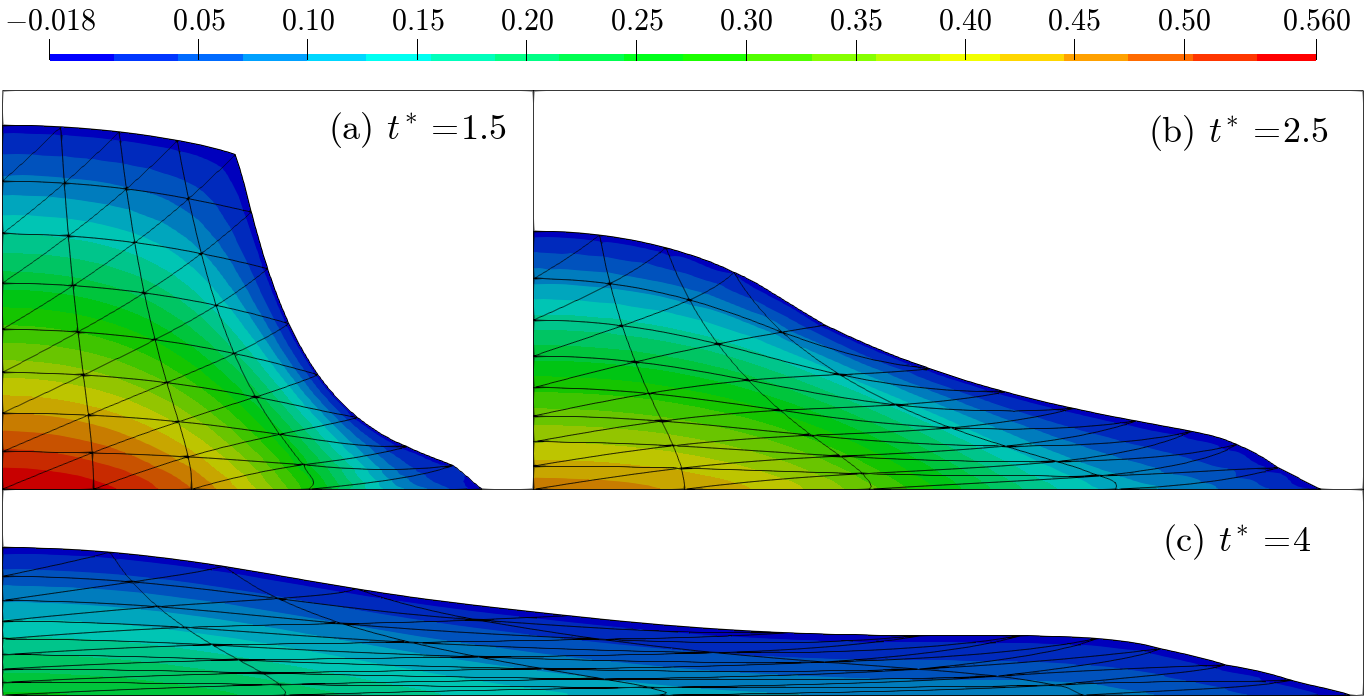
\includegraphics[scale=0.4]{Figuras/FluidDam/FluidDamT10.png}
	%\caption*{\textbf{Fonte:} Elaborado pelo autor}
\end{figure}

Na \autoref{fig:FluidDam-widthVariation} são apresentados os resultados de variação do comprimento e de pressão ao longo do tempo adimensional. O primeiro, apresentado na \autoref{fig:FluidDam-widthVariation}(a), é tomado como $L/L_0$, onde $L$ é a distância entre as extremidades inferiores esquerda e direita do domínio em cada passo de tempo, e $L_0 = 0,35$m é o comprimento original da coluna de água. O gráfico obtido é comparado com os resultados numéricos de \citeonline{Nithiarasu2005} e com os experimentais de \citeonline{Martin1952PartIA}, mostrando uma excelente concordância. Já a pressão, apresentada na \autoref{fig:FluidDam-widthVariation}(b), é medida na extremidade inferior esquerda do domínio, e é comparada com os resultados numéricos de \citeonline{Avancini2020}, mostrando também concordância satisfatória.

\begin{figure}[!htb]
	\centering
	\caption{Gráficos ao longo do tempo adimensional de (a) Variação do comprimento do domínio e (b) Pressão medida no ponto inferior esquerdo}
	\label{fig:FluidDam-widthVariation}
	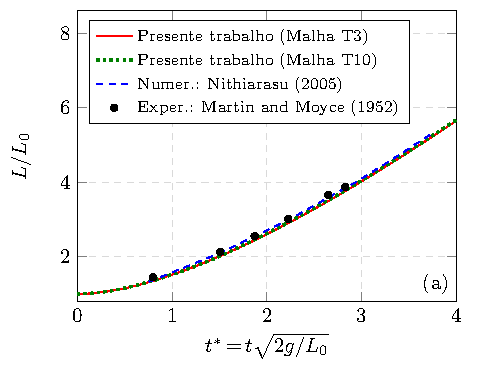
\includegraphics[scale=1.0]{Figuras/FluidDam/FluidDam-widthVariation.pdf}\;\;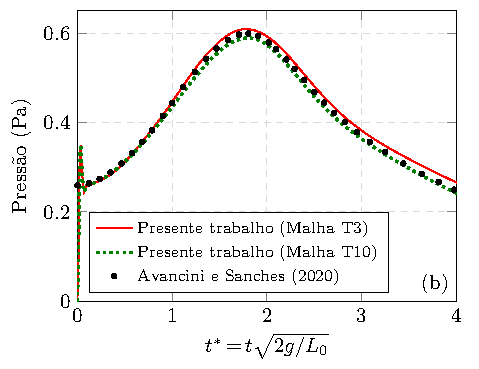
\includegraphics[scale=1.0]{Figuras/FluidDam/FluidDam-pressure.pdf}
	%\caption*{\textbf{Fonte:} Elaborado pelo autor}
\end{figure}

\subsubsection{Fluido sob tensão superficial: caso 2D}

Neste exemplo, analisamos o efeito da tensão superficial sobre um fluido Newtoniano incompressível com domínio inicial quadrilateral conforme a \cref{fig:SurfaceTension2D}. Devido à simetria do problema, apenas um quadrante do domínio é discretizado, aplicando-se as devidas condições de contorno nas interfaces com os eixos de simetria. Nenhuma força é aplicada no domínio além da tensão superficial $\surfaceTension$ prescrita no contorno externo. O valor de $\surfaceTension$ é considerado constante ao longo do contorno e do tempo. 

\begin{figure}[!htb]
	\centering
	\caption{Geometria e condições de contorno para exemplo de fluido sob tensão superficial em 2D}
	\label{fig:SurfaceTension2D}
	{\small
		\noindent\shadowbox{
			\parbox{15.3cm}{
				\setlength{\columnseprule}{1pt}
				\vspace{-0.2cm}
				{\centering\begin{center}
						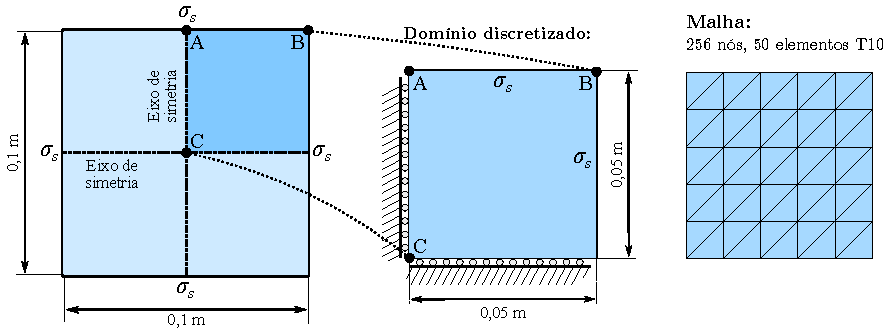
\includegraphics[scale=1]{Figuras/SurfaceTension2D/SurfaceTension2D.pdf}
					\end{center}\par}
				\vspace{-0.2cm}
			}
		}
	}	
	%\caption*{\textbf{Fonte:} Elaborado pelo autor}
\end{figure}

Para a discretização espacial, emprega-se uma malha regular composta por 50 elementos finitos do tipo T10. Para a discretização temporal, consideram-se $4000$ passos de tempo com $\Delta t = 2,5\cdot 10^{-3}$ s, e utiliza-se o integrador de Newmark-$\beta$ com parâmetros $\betanewmark = 1$ e $\gammanewmark = 1,5$. Além disso, aplica-se a estabilização PSPG neste exemplo, sendo o parâmetro $\multiplierpspg$ da \cref{eq:tpspg} tomado igual a $1000$.

A fim de verificar o comportamento do problema em diversas situações, múltiplas análises são realizadas, variando três parâmetros: a viscosidade ($\viscfluid$), a massa específica ($\massi$ ou $\mass$), e a tensão superficial ($\surfaceTension$).

Inicialmente, fixamos os parâmetros $\mass = 1$~kg/m$^3$ e $\surfaceTension = 10^{-4}$~N/m$^2$, e variamos o parâmetro de viscosidade em cinco casos: $1\cdot 10^{-2}$, $5\cdot 10^{-3}$, $1\cdot 10^{-3}$, $5\cdot 10^{-4}$ e $1\cdot 10^{-4}$ N$\cdot$s. A \cref{fig:FluidDrop-viscosity} mostra, para cada um desses casos, a evolução da distância entre os pontos A e C (indicados na \cref{fig:SurfaceTension2D}) e a pressão no ponto C. Além disso, as \cref{fig:FluidDrop-v1e-3,fig:FluidDrop-v5e-4,fig:FluidDrop-v1e-4} mostram as configurações deformadas em determinados instantes para três casos distintos de viscosidade, com campo de pressão ilustrado em mapa de cores.

\begin{figure}[!htb]
	\centering
	\caption{Gráficos ao longo do tempo de (a) distância entre pontos A e C, e (b) Pressão medida no ponto C, considerando diferentes valores de viscosidade}
	\label{fig:FluidDrop-viscosity}
	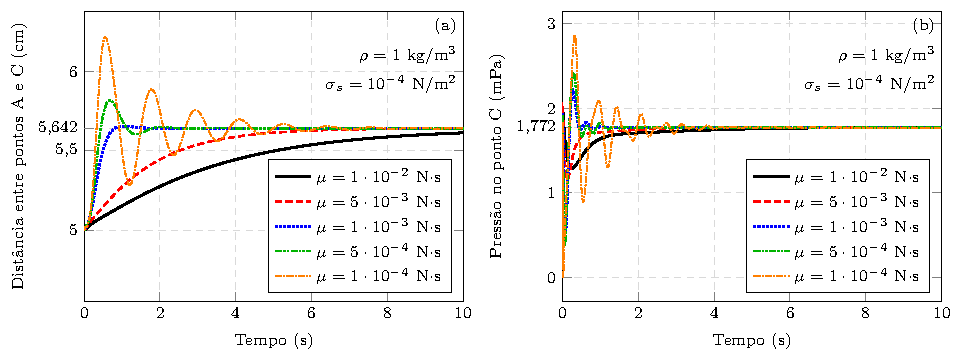
\includegraphics[scale=1.0]{Figuras/SurfaceTension2D/SurfaceTension2D-viscosity.pdf}
	%\caption*{\textbf{Fonte:} Elaborado pelo autor}
\end{figure}



\begin{figure}[!htb]
	\centering
	\caption{Configurações deformadas com pressão (Pa) em mapa de cores para o caso com $\viscfluid = 10^{-3}$~N$\cdot$s, $\mass = 1$~kg/m$^3$ e $\surfaceTension = 10^{-4}$~N/m$^2$}
	\label{fig:FluidDrop-v1e-3}
	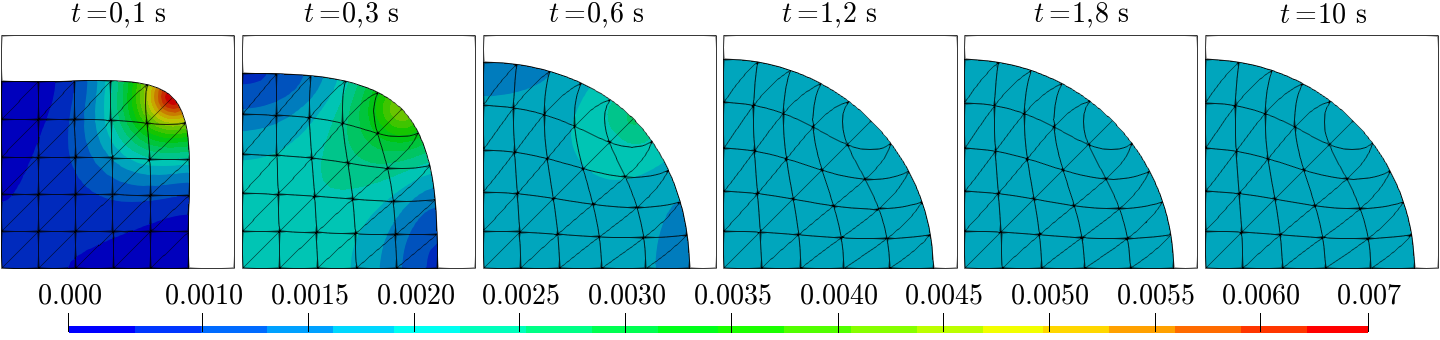
\includegraphics[scale=0.42]{Figuras/SurfaceTension2D/Paraview/v1e-3.png}
	%\caption*{\textbf{Fonte:} Elaborado pelo autor}
\end{figure}

\begin{figure}[!htb]
	\centering
	\caption{Configurações deformadas com pressão (Pa) em mapa de cores para o caso com $\viscfluid=5\cdot10^{-4}$~N$\cdot$s, $\mass = 1$~kg/m$^3$ e $\surfaceTension = 10^{-4}$~N/m$^2$}
	\label{fig:FluidDrop-v5e-4}
	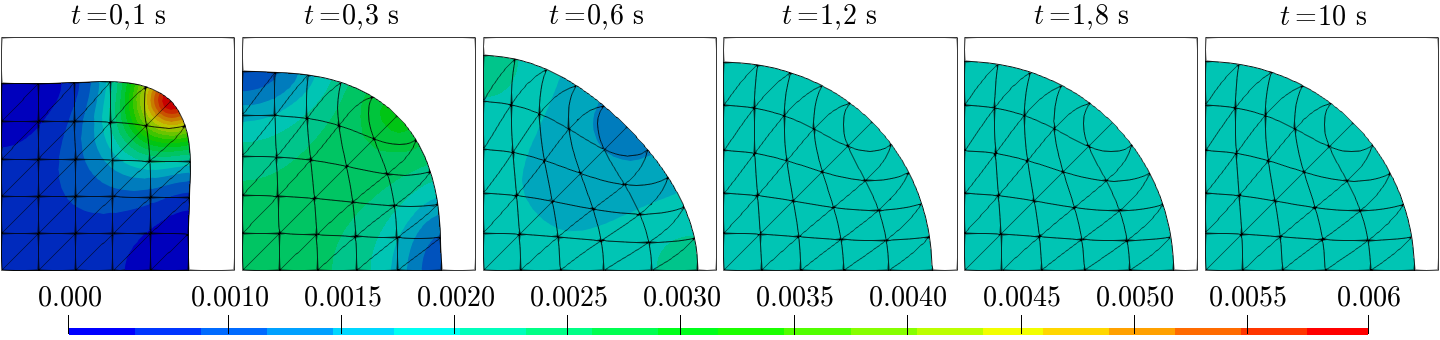
\includegraphics[scale=0.42]{Figuras/SurfaceTension2D/Paraview/v5e-4.png}
	%\caption*{\textbf{Fonte:} Elaborado pelo autor}
\end{figure}

\begin{figure}[!htb]
	\centering
	\caption{Configurações deformadas com pressão (Pa) em mapa de cores para o caso com $\viscfluid = 10^{-4}$~N$\cdot$s, $\mass = 1$~kg/m$^3$ e $\surfaceTension = 10^{-4}$~N/m$^2$}
	\label{fig:FluidDrop-v1e-4}
	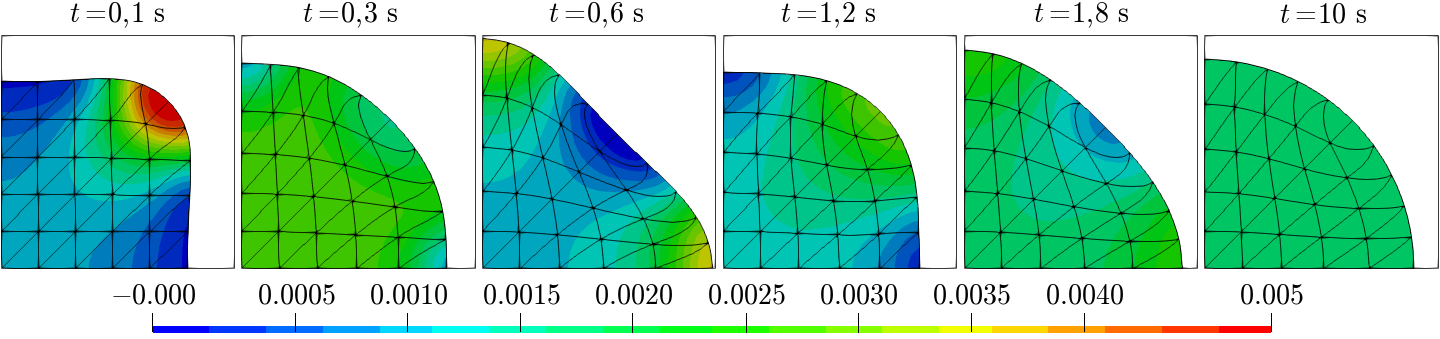
\includegraphics[scale=0.42]{Figuras/SurfaceTension2D/Paraview/v1e-4.png}
	%\caption*{\textbf{Fonte:} Elaborado pelo autor}
\end{figure}

Conforme discutido na \cref{subsec:forcas-tensao-residual}, a tensão superficial tende a minimizar a área da superfície para um dado volume fixo (ou área fixa, no caso 2D), fazendo com que o domínio inicialmente quadrilateral adquira uma forma circular à medida que o tempo avança. Essa tendência pode ser observada em todos os casos analisados, embora o comportamento do material até atingir sua forma estabilizada varie de acordo com os parâmetros adotados. 

A variação da viscosidade, por exemplo, influencia diretamente no perfil oscilatório do material. Como pode ser notado nas \cref{fig:FluidDrop-viscosity,fig:FluidDrop-v1e-3,fig:FluidDrop-v5e-4,fig:FluidDrop-v1e-4}, os casos com menor viscosidade tendem a oscilar mais antes de estabilizar, enquanto os casos com maior viscosidade apresentam uma convergência mais suave, sendo mais lenta conforme o parâmetro $\viscfluid$ aumenta.

Como o material é incompressível, a área do do quadrante discretizado ($A=0,05^2 = 2,5\cdot 10^{-3}$ m$^2$) é mantida fixa durante o processo. Assim, é possível calcular de forma analítica o raio do círculo resultante como $R=\sqrt{4A/\pi}\approx 0,0564$~m. É possível observar na \cref{fig:FluidDrop-viscosity}(a) que a distância entre os pontos A e C tende para esse raio, independentemente do perfil oscilatório, o que demonstra uma coerência nos resultados.

Sabendo que a curvatura média de um cilindro é $\curvature = 1/(2R)$, também podemos calcular a pressão resultante no domínio de forma analítica como $p = 2\surfaceTension\curvature = \surfaceTension/R$. Com $\surfaceTension = 10^{-4}$~N/m$^2$, obtemos $p \approx 0,001772$ Pa. Novamente, constatamos que as pressões na \cref{fig:FluidDrop-viscosity}(b) tendem para esse valor, reforçando a consistência do modelo.


Seguindo para uma segunda análise, avaliamos a influência da massa específica sobre o problema. Neste caso, fixamos os parâmetros $\viscfluid$ e $\surfaceTension$, e variamos $\massi$ em três casos: $4$, $2$ e $1$ kg/m$^3$. Os gráficos resultantes dessa análise para $\viscfluid = 10^{-4}$~N$\cdot$s e $\surfaceTension = 10^{-4}$~N/m$^2$ são apresentados na \cref{fig:FluidDrop-mass}, e para $\viscfluid = 5\cdot 10^{-3}$~N$\cdot$s e $\surfaceTension = 10^{-4}$~N/m$^2$ são apresentados na \cref{fig:FluidDrop-mass3}. 

\begin{figure}[!htb]
	\centering
	\caption{Gráficos ao longo do tempo de (a) distância entre pontos A e C, e (b) Pressão medida no ponto C, para $\viscfluid = 10^{-4}$~N$\cdot$s, $\surfaceTension = 10^{-4}$~N/m$^2$, e diferentes valores de massa específica}
	\label{fig:FluidDrop-mass}
	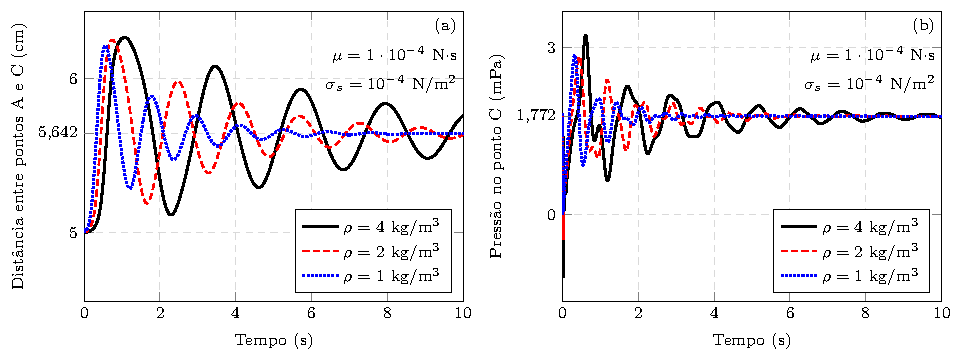
\includegraphics[scale=1.0]{Figuras/SurfaceTension2D/SurfaceTension2D-mass.pdf}
	%\caption*{\textbf{Fonte:} Elaborado pelo autor}
\end{figure}

\begin{figure}[!htb]
	\centering
	\caption{Gráficos ao longo do tempo de (a) distância entre pontos A e C, e (b) Pressão medida no ponto C, para $\viscfluid = 5\cdot 10^{-3}$~N$\cdot$s, $\surfaceTension = 10^{-4}$~N/m$^2$, e diferentes valores de massa específica}
	\label{fig:FluidDrop-mass3}
	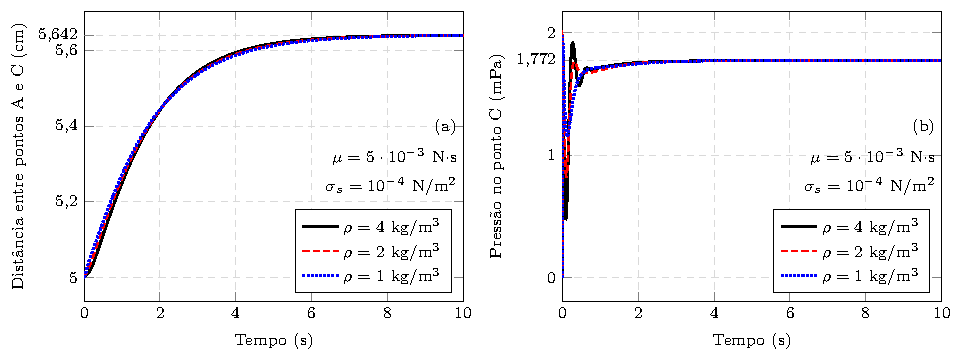
\includegraphics[scale=1.0]{Figuras/SurfaceTension2D/SurfaceTension2D-mass3.pdf}
	%\caption*{\textbf{Fonte:} Elaborado pelo autor}
\end{figure}


Como pode ser observado, a variação da massa específica não altera substancialmente o perfil oscilatório, mas impacta diretamente a frequência da oscilação, afetando assim o tempo necessário para estabilização quando a oscilação é mais pronunciada, como nos casos de baixa viscosidade. Dentre os gráficos apresentados na \cref{fig:FluidDrop-mass}, por exemplo, o menor tempo de estabilização foi obtido para $\mass = 1$ kg/m$^3$, enquanto os casos com valores mais altos de $\mass$ demandaram um tempo mais prolongado, sendo o período total considerado na análise ($10$ s) insuficiente para uma convergência satisfatória.

Já no caso da \cref{fig:FluidDrop-mass3}, onde a viscosidade é mais alta e a oscilação menos significativa, a variação da massa específica tem pouca influência nos resultados. Particularmente na \cref{fig:FluidDrop-mass3}(a), os gráficos demonstram comportamentos quase idênticos durante toda a análise. Na \cref{fig:FluidDrop-mass3}(b) também pode ser observada uma rápida convergência dos resultados, embora hajam algumas divergências no início da análise.

Por fim, analisamos a influência da tensão superficial sobre o problema. Neste caso, fixamos os parâmetros $\viscfluid$ e $\massi$, e variamos $\surfaceTension$ em três casos: $1\cdot 10^{-4}$, $5\cdot 10^{-5}$ e $1\cdot 10^{-5}$ N/m$^2$. Os gráficos resultantes para $\viscfluid = 10^{-4}$~N$\cdot$s e $\mass = 1$ kg/m$^3$ são apresentados na \cref{fig:FluidDrop-surfaceTension}, e para $\viscfluid = 5\cdot 10^{-3}$~N$\cdot$s e $\mass = 1$ kg/m$^3$ são apresentados na \cref{fig:FluidDrop-surfaceTension3}. 

\begin{figure}[!htb]
	\centering
	\caption{Gráficos ao longo do tempo de (a) distância entre pontos A e C, e (b) Pressão medida no ponto C, para $\viscfluid = 10^{-4}$~N$\cdot$s e $\mass = 1$ kg/m$^3$, e diferentes valores de tensão superficial}
	\label{fig:FluidDrop-surfaceTension}
	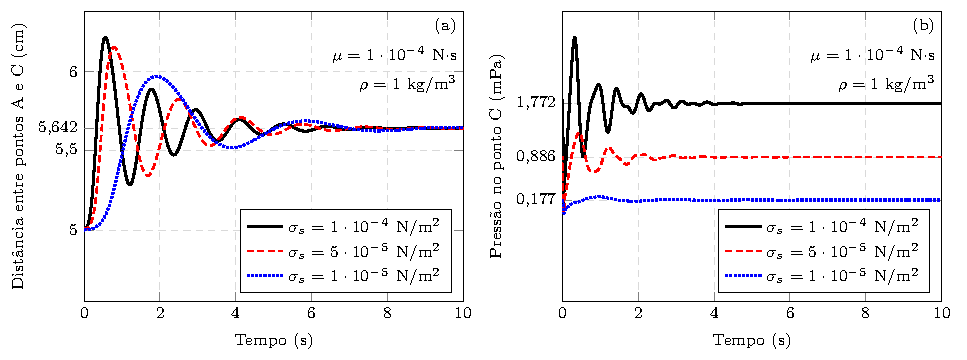
\includegraphics[scale=1.0]{Figuras/SurfaceTension2D/SurfaceTension2D-tension.pdf}
	%\caption*{\textbf{Fonte:} Elaborado pelo autor}
\end{figure}

\begin{figure}[!htb]
	\centering
	\caption{Gráficos ao longo do tempo de (a) distância entre pontos A e C, e (b) Pressão medida no ponto C, para $\viscfluid = 5\cdot 10^{-3}$~N$\cdot$s e $\mass = 1$ kg/m$^3$, e diferentes valores de tensão superficial}
	\label{fig:FluidDrop-surfaceTension3}
	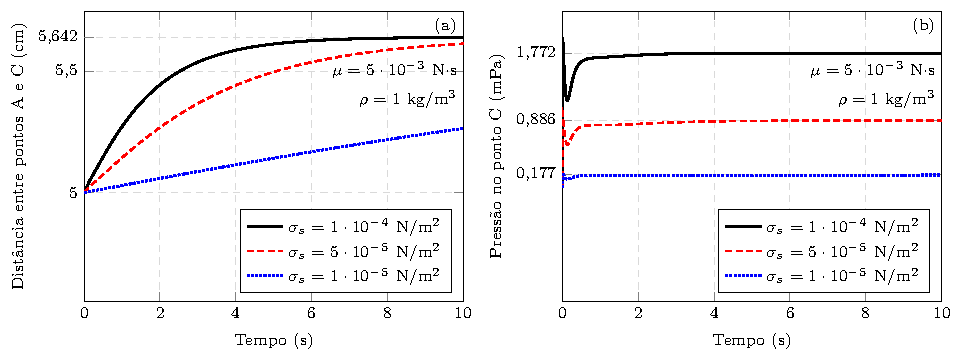
\includegraphics[scale=1.0]{Figuras/SurfaceTension2D/SurfaceTension2D-tension3.pdf}
	%\caption*{\textbf{Fonte:} Elaborado pelo autor}
\end{figure}

Embora o raio do círculo resultante não varie em função de $\surfaceTension$, nota-se que o valor estabilizado da pressão varia, uma vez que, conforme deduzido anteriormente, sua expressão analítica é $p = \surfaceTension/R$. Para os casos considerados de $\surfaceTension$, essa expressão resulta nos valores $1,772\cdot 10^{-3}$, $0,886\cdot 10^{-3}$ e $0,177\cdot 10^{-3}$ Pa, produzindo gráficos de pressão com alinhamentos distintos, como pode ser visto nas Figs. \ref{fig:FluidDrop-surfaceTension}(b) e \ref{fig:FluidDrop-surfaceTension3}(b).

Avaliando mais profundamente a influência de $\surfaceTension$ sobre os resultados, percebemos comportamentos distintos de acordo com o nível de viscosidade considerado. Para o caso com $\viscfluid = 10^{-4}$~N$\cdot$s, a variação de $\surfaceTension$ afeta a frequência das oscilações, mas não altera significativamente o tempo de estabilização. Já no caso com $\viscfluid = 5\cdot 10^{-3}$~N$\cdot$s, onde a viscosidade é suficientemente alta para que não sejam visíveis oscilações, o tempo de estabilização da distância entre os pontos A e C é fortemente influenciado pela tensão superficial, sendo mais longo conforme $\surfaceTension$ diminui. No entanto, esse comportamento não se generaliza para os gráficos de pressão, que convergem rapidamente para as respostas analíticas independentemente do valor de $\surfaceTension$.

\subsubsection{Fluido sob tensão superficial: caso 3D}

Para ilustrar o efeito da tensão superficial em um caso tridimensional, propõe-se nesta seção uma generalização do exemplo anterior, considerando um fluido Newtoniano incompressível com domínio inicial em forma de cubo, conforme a \cref{fig:SurfaceTension3D}. Utilizando novamente a simetria do problema, discretizamos apenas um octante do domínio, aplicando as condições de contorno apropriadas nas interfaces com os eixos de simetria. Neste caso, fixamos a tensão superficial no contorno externo em $\surfaceTension = 10^{-4}$~N/m$^2$, constante ao longo do tempo, e os parâmetros do material em $\viscfluid = 10^{-4}$~N$\cdot$s e $\massi = \mass = 1$~kg/m$^3$.

\begin{figure}[!htb]
	\centering
	\caption{Geometria e condições de contorno para exemplo de fluido sob tensão superficial em 3D}
	\label{fig:SurfaceTension3D}
	{\small
		\noindent\shadowbox{
			\parbox{15.3cm}{
				\setlength{\columnseprule}{1pt}
				\vspace{-0.2cm}
				{\centering\begin{center}
						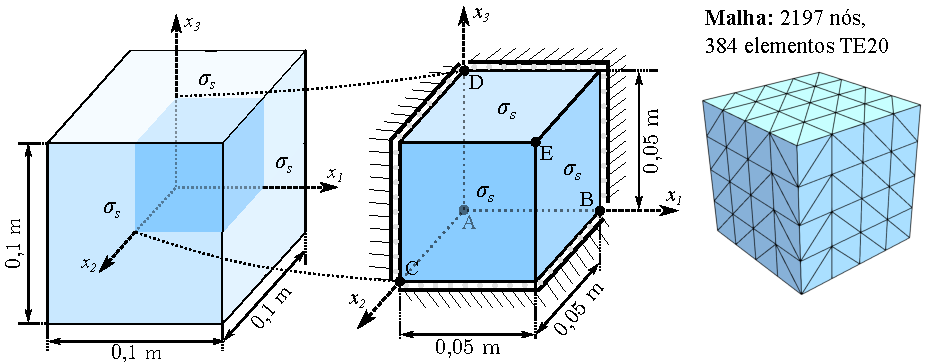
\includegraphics[scale=0.95]{Figuras/SurfaceTension3D/SurfaceTension3D.pdf}
					\end{center}\par}
				\vspace{-0.2cm}
			}
		}
	}	
	%\caption*{\textbf{Fonte:} Elaborado pelo autor}
\end{figure}

Utiliza-se uma malha regular composta por 384 elementos finitos tetraédricos de terceira ordem (TE20). Os demais parâmetros da análise são similares aos do exemplo anterior: $4000$ passos de tempo com $\Delta t = 2,5\cdot 10^{-3}$ s; integrador de Newmark-$\beta$ com parâmetros $\betanewmark = 1$ e $\gammanewmark = 1,5$; e estabilização PSPG com $\multiplierpspg = 1000$.

Na \cref{fig:FluidDrop3D-graphs}(a), avaliamos a distância entre diversos pontos do contorno externo (indicados na \cref{fig:SurfaceTension3D}) e o centro do domínio (ponto A). Na \cref{fig:FluidDrop3D-graphs}(b), são apresentados os gráficos de pressão ao longo do tempo para os mesmos pontos. Por fim, na \cref{fig:FluidDrop3D}, ilustramos as configurações deformadas do domínio discretizado em determinados instantes da análise, com campo de pressão em mapa de cores.

\begin{figure}[!htb]
	\centering
	\caption{Gráficos de (a) distância ao ponto A e (b) pressão, para diversos pontos do contorno sob tensão superficial em 3D}
	\label{fig:FluidDrop3D-graphs}
	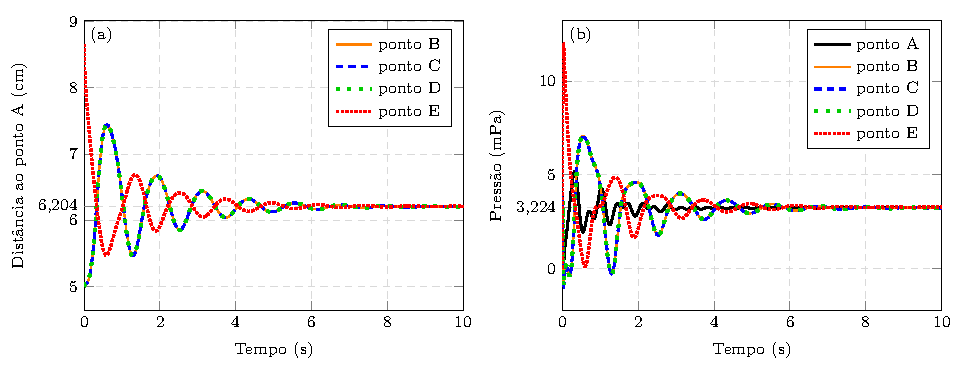
\includegraphics[scale=1.0]{Figuras/SurfaceTension3D/SurfaceTension3D-graph.pdf}
	%\caption*{\textbf{Fonte:} Elaborado pelo autor}
\end{figure}

\begin{figure}[!htb]
	\centering
	\caption{Configurações deformadas com pressão (Pa) em mapa de cores para o exemplo de fluido sob tensão superficial em 3D}
	\label{fig:FluidDrop3D}
	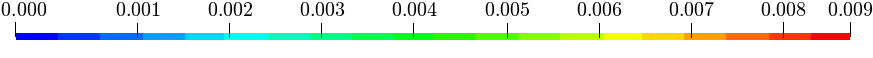
\includegraphics[scale=0.6]{Figuras/SurfaceTension3D/Paraview/legend.png}
	
	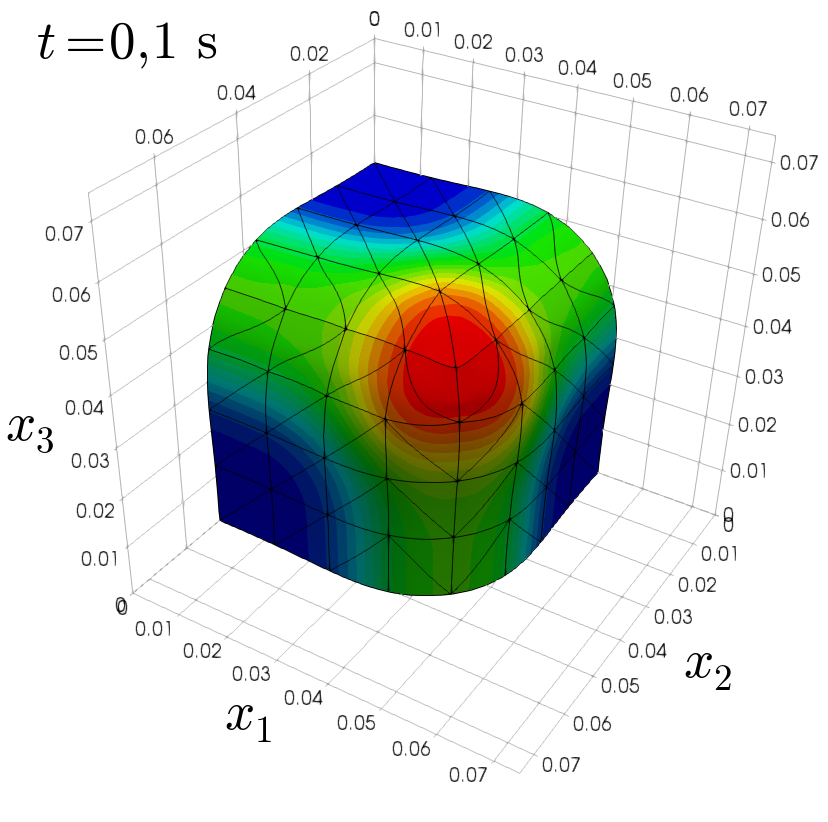
\includegraphics[scale=0.18]{Figuras/SurfaceTension3D/Paraview/t1.png}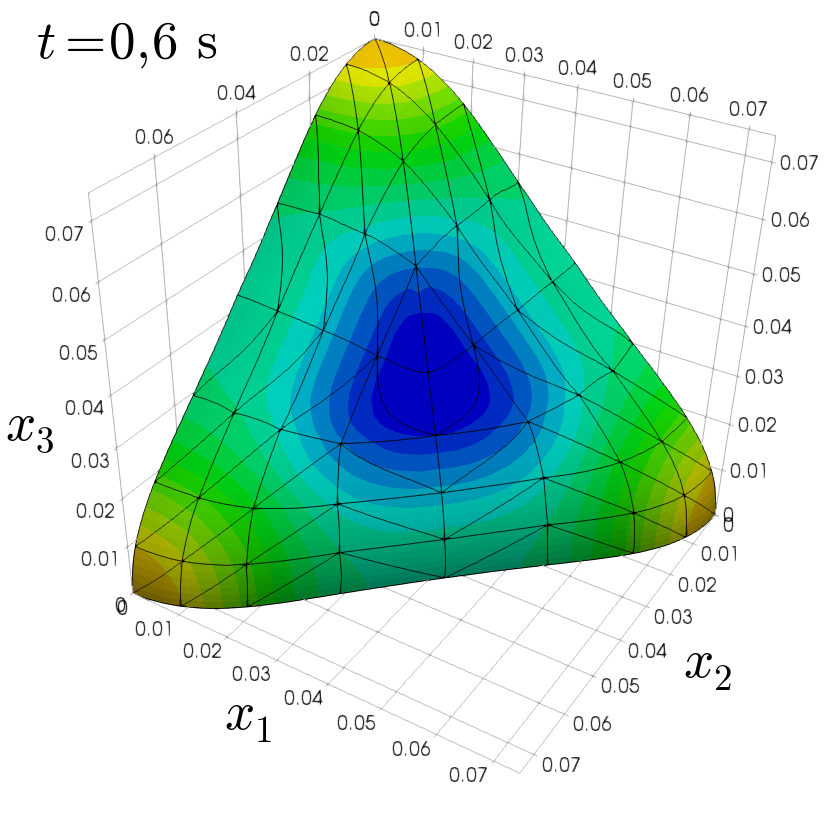
\includegraphics[scale=0.18]{Figuras/SurfaceTension3D/Paraview/t6.png}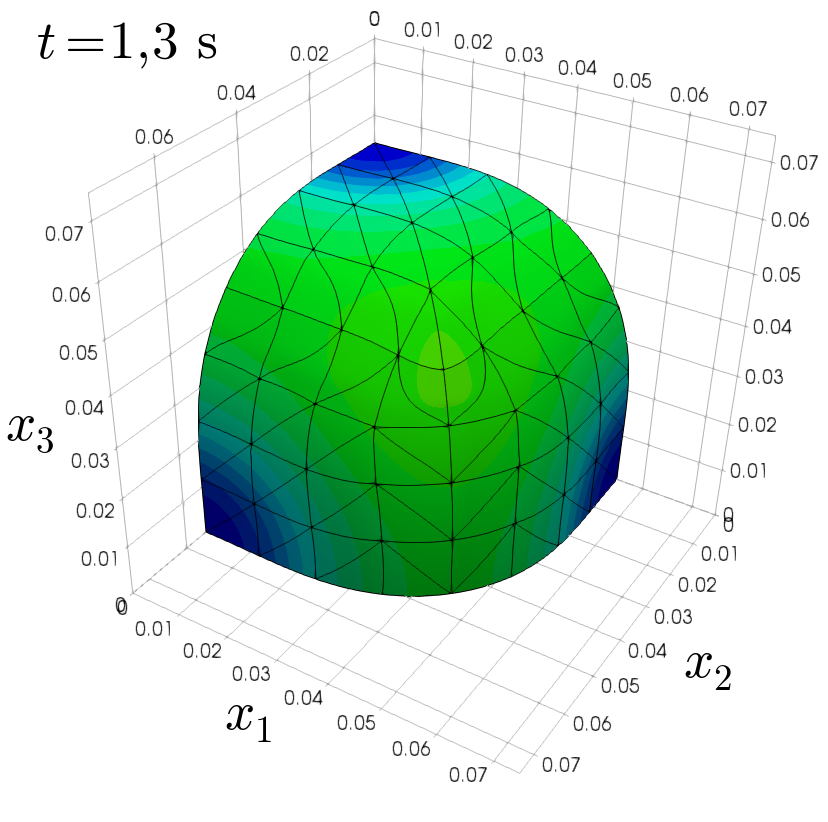
\includegraphics[scale=0.18]{Figuras/SurfaceTension3D/Paraview/t13.png}
	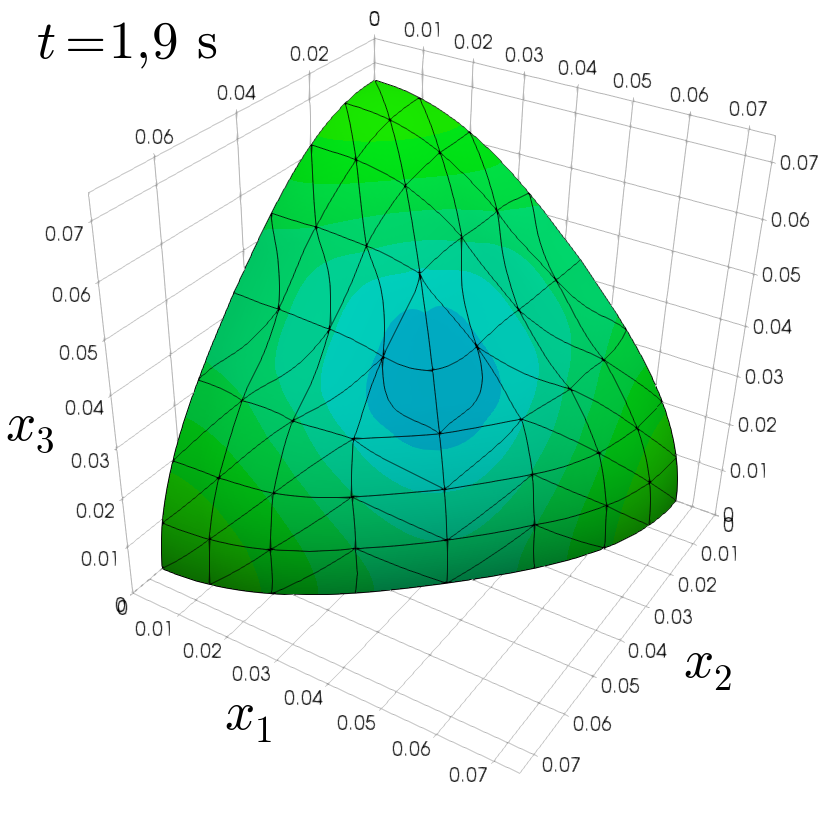
\includegraphics[scale=0.18]{Figuras/SurfaceTension3D/Paraview/t19.png}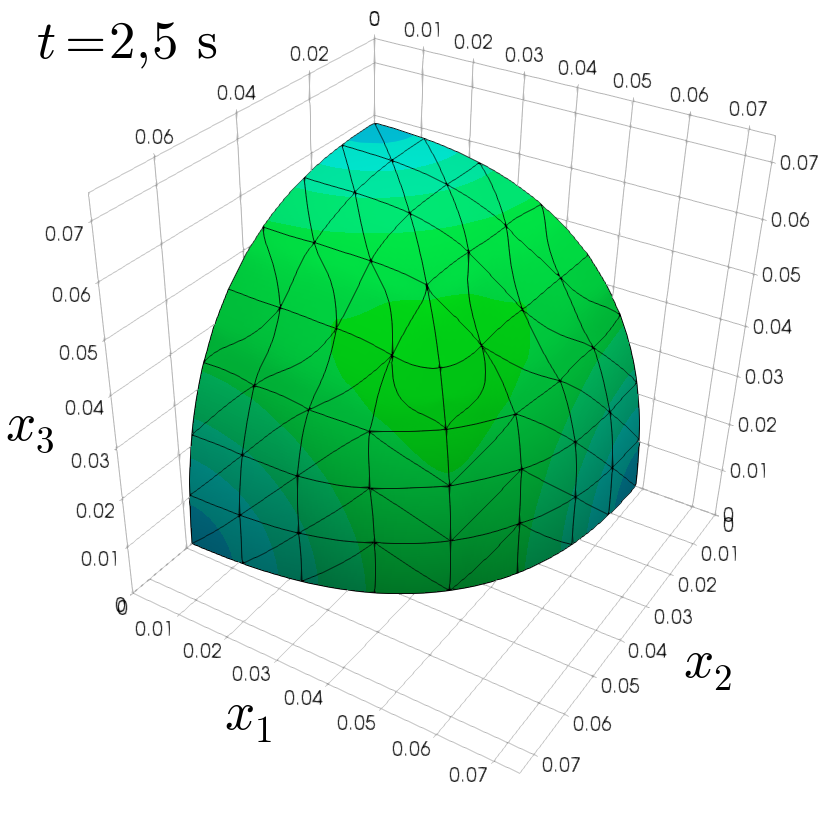
\includegraphics[scale=0.18]{Figuras/SurfaceTension3D/Paraview/t25.png}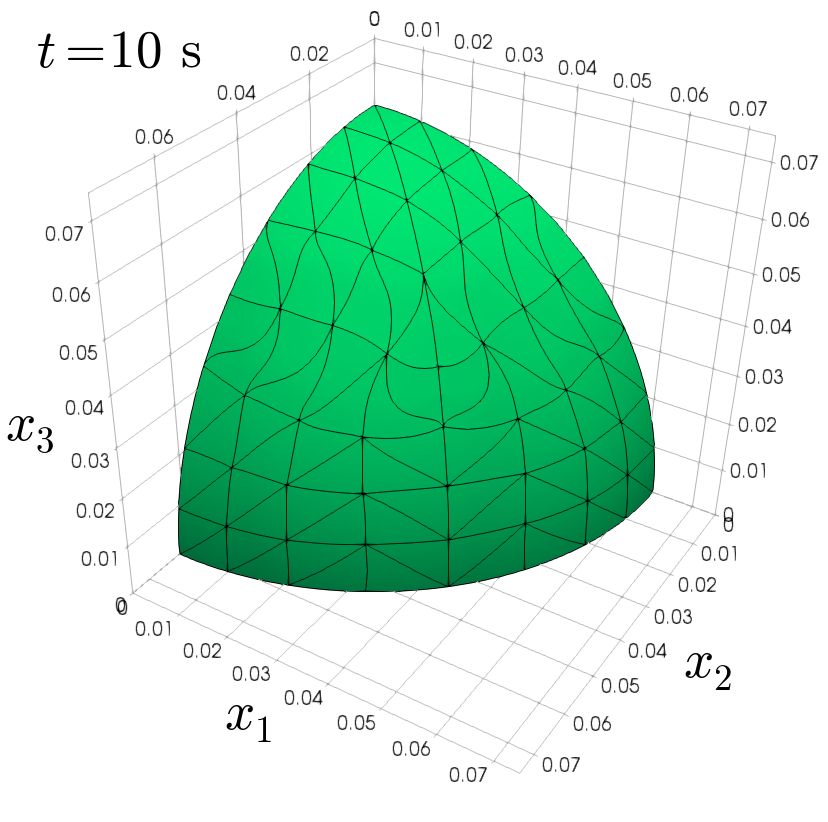
\includegraphics[scale=0.18]{Figuras/SurfaceTension3D/Paraview/t100.png}
	%\caption*{\textbf{Fonte:} Elaborado pelo autor}
\end{figure}

Podemos observar novamente um comportamento oscilatório com estabilização gradual. Neste caso, o efeito da tensão superficial faz com que a forma cúbica do domínio tenda a assumir uma configuração esférica. Dada a incompressibilidade do material, o volume do octante discretizado ($V = 0,05^3 = 1,25\cdot 10^{-4}$~m$^3$) é mantido fixo ao longo do processo. Assim, podemos calcular o raio da esfera resultante analiticamente como $R = \sqrt[3]{6V/\pi} \approx 0,06204$~m. Como a curvatura média da esfera é $1/R$, a pressão resultante no domínio também pode ser calculada de forma analítica como $p = 2\surfaceTension\curvature = 2\surfaceTension/R \approx 3,224\cdot 10^{-3}$~Pa. Nota-se que, na \cref{fig:FluidDrop3D-graphs}, as pressões tendem a esse valor, e os gráficos das distâncias medidas tendem ao raio previamente calculado, demonstrando a consistência dos resultados obtidos.


\end{document}